% ****** Start of file apssamp.tex ******
%
%   This file is part of the APS files in the REVTeX 4.2 distribution.
%   Version 4.2a of REVTeX, December 2014
%
%   Copyright (c) 2014 The American Physical Society.
%
%   See the REVTeX 4 README file for restrictions and more information.
%
% TeX'ing this file requires that you have AMS-LaTeX 2.0 installed
% as well as the rest of the prerequisites for REVTeX 4.2
%
% See the REVTeX 4 README file
% It also requires running BibTeX. The commands are as follows:
%
%  1)  latex apssamp.tex
%  2)  bibtex apssamp
%  3)  latex apssamp.tex
%  4)  latex apssamp.tex
%
\documentclass[%
 reprint,
%superscriptaddress,
%groupedaddress,
%unsortedaddress,
%runinaddress,
%frontmatterverbose, 
%preprint,
%preprintnumbers,
%nofootinbib,
%nobibnotes,
%bibnotes,
 amsmath,amssymb,
 aps,
%pra,
%prb,
%rmp,
%prstab,
%prstper,
%floatfix,
]{revtex4-2}
\usepackage{enumitem}
\usepackage{graphicx}% Include figure files
\usepackage{dcolumn}% Align table columns on decimal point
\usepackage{bm}% bold math
\usepackage{braket}
%\usepackage{hyperref}% add hypertext capabilities
%\usepackage[mathlines]{lineno}% Enable numbering of text and display math
%\linenumbers\relax % Commence numbering lines

%\usepackage[showframe,%Uncomment any one of the following lines to test 
%%scale=0.7, marginratio={1:1, 2:3}, ignoreall,% default settings
%%text={7in,10in},centering,
%%margin=1.5in,
%%total={6.5in,8.75in}, top=1.2in, left=0.9in, includefoot,
%%height=10in,a5paper,hmargin={3cm,0.8in},
%]{geometry}
\allowdisplaybreaks

\begin{document}

\preprint{APS/123-QED}

\title{Quantum well structure and nonlinear absorption interaction - a review}% Force line breaks with \\
\thanks{Low-dimensional semiconductor-based theoretical structures.}%

\author{Khanh Gia Bui}
 %\altaffiliation[Also at ]{Physics Department, XYZ University.}%Lines break automatically or can be forced with \\
\author{Khoa Ngoc Duong}%
\author{Duc Phung Nguyen}
 %\email{Second.Author@institution.edu}
\affiliation{%
Department of Physics, Hanoi University of Science \\
  Hanoi, Vietnam
}%

%\collaboration{MUSO Collaboration}%\noaffiliation

%\author{Duc Phung Nguyen}
% \homepage{https://amane-fujimiya.github.io/about/about.html}
%\affiliation{
% Second institution and/or address\\
% This line break forced% with \\
%}%
%\affiliation{
% Third institution, the second for Charlie Author
%}%
%\author{Delta Author}
%\affiliation{%
% Authors' institution and/or address\\
% 
%}%

%\collaboration{CLEO Collaboration}%\noaffiliation

\date{\today}% It is always \today, today,
             %  but any date may be explicitly specified

\begin{abstract}
In this paper, we provide non-original analysis and historical coverage on the topic of quantum well and system utilizing it, the foundational reason for such model, and the physical systems interpretation of such quantum theory. Furthermore, we would like to give an example on the consideration of \textit{nonlinear absorption effect} in such system, for the example of half-parabolic, asymmetric, finite, additive quantum well with or without the presence of a uniform electric field of perpendicular sectioning in the $z$-axis. The scope of the origin of quantum well and necessity of such modelling will also be included of typical geometrical configuration of a low-dimensional restrictive well.  
\end{abstract}

%\keywords{Suggested keywords}%Use showkeys class option if keyword
                              %display desired
\maketitle

%\tableofcontents

\section{Introduction}

Quantum well, or rather, specified topology on coordinate space of specific mechanistic landscapes, has been one of the central part in the framework of quantum mechanics. Indeed, foundational sources, textbooks and materials in quantum physics considers different forms of such quantum confinement environment as to gauge how a non-free space system evolutes and changes, which align with much of the observable results. While textbooks and works \cite{griffiths2018,sakurai2017,landau1981} has been introducing the concepts and working of quantum potential confinement and so on, the inner working of systems in practical setting or of more complicated requirements, such as semiconductors and typical design space, as seen of historical works or textbooks \cite{kane1957,chang1980,kittel2005,bastard1988,davies1998,harrison2016,weisbuch1991,haugkoch2009,yu2010,barsan2016,esaki1974}, and require much more sophisticated mechanisms or theoretical tooling to work. As such, we are inclined to provide a partial analysis of target, on the structure and treatment of \textit{quantum confinement structures}, and the deliberate exact analytical results and limitation in forcing such approach. 

Furthermore, as noted, the subject is very complex with multiple structures existing and adding together in a large form. Such includes, for example, \textit{effective-mass} formulation, \textit{k-p perturbation theory} and \textit{envelope-function approximation}, and so on, we would like to review through the situation and justification of using the frameworks. Inherently, they are effective but imperfect formulation, such is also why new developments are being developed to fill in their gaps. Nevertheless, the analysis aims to clarify such hedging space, and furthermore to utilize the existing theory to its effect as is. 

\section{Preliminary}

Quantum well structure branched out from quantum theory, and the typical potential insertion as a more practical, or more physically relevant model of considering real system beyond finite and infinite well. As such, currently, they are more correlated to be defined as \textit{thin layered semiconductor structures} in which we can observe and control quantum mechanical effects, all of which are non-free particle system of which can be naturally said of to be the ambiance \textbf{topology} of the physical system itself (per Schrödinger equation expression and so on). As such, per David A. B. Miller \cite{David2020OpticalPO}, the quantum well structure and its relevant class of restriction (quantum wire and quantum dot) derive most of their special properties from "the quantum confinement of charge carriers in thin layers, of one semiconductor well material sandwiched between other semiconductor barrier layers". If the middle layer is effectively non-impeding in any sense, be it vacuum or transmittable medium, the topology is analogous to square potential restriction, of which is analogous to quantum potential models in theory. They are useful, as laboratory setting in which can be used to set up much more complicated structures or setting, with feasibility of mechanism control than directly observe, for example, excitons at large. In essence, we can say that quantum well or potential-induced structures, makes up the bulk of relevant topology-creating physical system quantum theory most often consider itself in of scale; and simply speak, quantum theory becomes physically meaningful only once a potential defines structural topology to work on it. The easiest justification of such, is from the observation of the fact that in the current model, all nontrivial quantum topology enters through constraints on the Hamiltonian.

We would like to clarify the usage of \textbf{topology} here is rather non-standard, and would clash with typical intuition on algebraic or differential topology, and so on. The usage here is rather \textbf{ontological} in its core argument, and it puts the physical reality on the \textbf{first-order} basis (highest) \footnote{The need for this clarification is justified, as for even sophisticated reader, and a lot of Large Language Model (LLM) of existence, failed to read this part, or discard it as unimportant directly, and criticize it later on. In a sense, automated machines or formalist readers systematically discard ontological framing and then retroactively impose mathematical standards, which is what we are to prevent our interpretation to be of.}. Thus, while sharing the naming, rather, what we want to emphasize here is the definition on which hinges on the onset of, for example in this relevant context, \textit{how the Hamiltonian carves out configuration space and Hilbert space} into allowed and forbidden regions, or rather, what exists before a theory, or treatment, can talk about representation on smoothness, manifolds, or bundles, that are justified or not. In such sense, topology here is \textbf{first-order}, basing the system in consideration of all admissible solutions first and foremost, and is created from confinement, boundary, or periodic conditions, and domain restriction of operators. It is then closer to spectral topology, or operator-domain topology than to differential topology, of which would be considered in such case to be the \textbf{second-order topology}, induced by mathematical structures in interpretation of the configuration space. Naturally, the usage would be fairly standard once it is clarified. In Schrödinger theory or to the larger degree of quantum theory, there are normally three structural inputs that shape the system. First is the base space, which is usually $\mathbb{R}^{n}$, the Hamiltonian operator, and the domain on which that operator is self-adjoint to be of interest. As such, in the expression of the Schrödinger equation, $V(x)$ is the most important external fixture of which applies on all three. Dirac equation inherits the same topology, but with added first or second-order topology only, for example, the \textbf{spinor topology}, relativistic dispersion, or gauge coupling as geometric potential. In practice, especially for structure of interest, Dirac equation is reduced back to Schrodinger-type envelope equations via nonrelativistic limits or Foldy-Wouthuysen transformations, which reduces the equation to Schrödinger-Pauli equation. In fact, by observation, the Schrödinger equation,
\begin{equation}
    i\hbar \partial_{t}\psi = \left(-\frac{\hbar^2}{2m}\nabla^{2}+V(x)\right)\psi
\end{equation}
and the Dirac equation on relativistic formulation,
\begin{equation}
    i\hbar \partial_t \Psi = (-i\hbar \bm{\alpha}\cdot \nabla + \beta mc^{2}+ V(x))\Psi
\end{equation}
share the same $V(x)$ external topology generation. Naturally so, we simply mean topology here as \textit{the constraint-induced structure of the quantum state space}. 

While the infinite well is a mathematical idealisation (hard walls, zero penetration); and the idealized theoretical finite well adds tunnelling and leakage, which is physically relevant when barriers are comparable to particle energy; the practical picture is rather much more different and complex, specifically considered of the potential resides inside the well, $V(x)$, and the shape of the barrier with admissible interaction. As such, the creation of models and explicit structures that can be replicated of such potential device, hinges on the goal for examining those conditions of the quantum system where their shapes are not trivial, and can induce complex interaction patterns, for example, \textit{nonlinear absorption} inside crystal lattices, all of which can be practically observed, or made to be near-approximation of ideal cases. From such goal, we also discovered, or rather made use of many contingent structures or interesting ordering beyond simply a single-potential system (in reality, such confinement in singularity is rather hard to make), for example, replacing isolated wells by a periodic atomic array, which leads to the concept of \textit{band formation} in such specific structural containment. The earliest example of this is from Kronig-Penney model \cite{10.1098/rspa.1931.0019}, of which studies the square-well periodic potential system. Such system considers
\begin{equation}
    V(x) = \begin{cases}
        V_{0} & -b \leq x \leq 0 \\
        0 & 0 < x \leq a
    \end{cases}
    , \quad 
    \psi(x+c) = \beta\psi(x)
\end{equation}

where $\beta$ is the constant of magnitude unity, or $\beta=\exp{(2\pi i l /n)}$, for $l=0,1,\dots,n-1$, and $c=a+b$ as the periodic length of the potential. The periodic property of the model can also be expressed as
\begin{equation}
    \psi(x+c) = e^{i\kappa c}\psi(x), \quad \kappa = 2\pi l/nc
\end{equation}
with nondimensionalization (for more, see \cite{li2024onedimensionperiodicpotentialsschrodinger} for also a fairly modern way of solving such system via finite difference method). Overall, the formulation started the conceptual bridge from single well to bulk semiconductor electronic structure, and thus enable the further road to actualize such well, and extending the topological formation system into much more active and sophisticated platforms. 

\subsection{Conductive and semiconductor}

The realization of quantum well, and later low-dimensional devices being created from conductive-capable or semiconductive materials, is rather an important step. Shifts to designing more sophisticated structures and topology is influenced by the capacity to actualize them on true physical devices, and hence, we are to give requirement to examine how the devices can form capture topology, and how they are used. Naturally, it also is not a one-way road, as understanding confining potential well topology helps in analysing well structures and material properties, and thus design philosophy. For a simple example, such is why there has been surges in the early 2000s for theoretical analysis on low-dimensional confining analysis, to analyse different properties of \textbf{Graphite}-based devices, mostly within nonlinear absorption phenomena, where conductivity of semiconductors can vary with environmental parameters, like temperature, light or electric current, with specifically important application as \textbf{optical computing}, and \textbf{optoelectronic devices}. 

It is then our task to provide a quick overview on how semiconductor device works, and the process in obtaining our quantum well confinement devices. Within such, we will develop an intuition on how the system is modelled, and to befit our experiences afterward. 

Semiconductor is constructed from solid-state material and structures. As said the topology of such material, for example, crystalline or at least solid lattice, creates \textbf{electronic behaviours} from electrons occupying energy bands inside, which are much closer than normal discretized energy level \cite{huang2DSemiconductorsSpecific2022}. Thence, at least for now, properties of solid, including \textit{doping} on shifted Fermi level, mechanical, thermal, fabrication scalability and stability, are what driving the usage of semiconductor in solid. While organic and molecular semiconductors \cite{FACCHETTI200728}, molecular electronics, and iontronics or bio-ionic devices are in rather active research, they cannot yet replace semiconductor for solid-state physics. Hence, for now, we would be fixed to this. 

Solid-states materials can be categorized into three classes - insulators, semiconductors, and conductors. They are categorized based on resistivity and conductivity, thus there are usually no fixed choice, for example as hydrogen being the standard baseline of molecular structure (as most analysis focused on them), but rather on what kind of compounds or element fits onto such category. Typical fit for semiconductor is with binary III-V columns semiconductor, or silicon and germanium single-element semiconductor. For semiconductor specifically, separation of bands happens when there exists more than two atoms together in interaction. Take Bohr model for example. The energy levels of a hydrogen atom are given by
\begin{equation}
    E_{H} = \frac{m_{o}q^{4}}{8\epsilon_{o}^{2}h^{2}n^2}
\end{equation}
for $m_{o}$ the free electron mass, $q$ the electron charge, $\epsilon_{o}$ the free space permittivity, $n$ the principle quantum number of the atom, and $h$ the Planck constant. By Heitler-London picture, when two hydrogens atoms $A$ and $B$ approach, each isolated \texttt{1s} level (note that this is much more general as for \textit{all electron in interaction}, hydrogen is the special case), $\ket{\phi_{A}}$ and $\ket{\phi_{B}}$ interacts through the two-electron Hamiltonian,
\begin{equation}
    \hat{H} = \hat{H}_{A} + \hat{H}_{B} + \hat{V}_{AB}
\end{equation}
for $\hat{V}_{AB}$ the Coulomb interactions between electrons and between electrons and the far nucleus. The molecular states specified thence reduces to
\begin{equation}
    \ket{\phi_{\pm}} = \frac{1}{\sqrt{2(1\pm \braket{\phi_{A}|\phi_{B}})}}(\ket{\phi_{A}\phi_{B}}\pm\phi_{B}\phi_{A})
\end{equation}
and solving this gives us the energy level description,
\begin{equation}
    E_{\pm} = \frac{E_{0}\pm H_{AB}}{1\pm \braket{\phi_{A}|\phi_{B}}}
\end{equation}
where $E_{0}$ is now the isolated atomic level, and $H_{AB}$ is expressed into the interaction matrix element. This allows the splitting of energy level in hydrogen, which is
\begin{equation}
    E_{+} - E_{-} \approx 2H_{AB} = 2 \braket{\phi_{A}|\hat{H}|\phi_{B}}
\end{equation}
This result is the basis for both Heitler-London and Slater-Pauling molecular orbital theory, and thus precedent to explain the splitting of such. For historical primary sources, see Heitler-London paper \cite{HeitlerLondon1927}, Slater and Koster's paper \cite{SlaterKoster1954} for Slater-Koster parameterization, and development, derivation of such results \cite{Papaconstantopoulos2003,Harrison1980,AshcroftMermin1976,kittel2005,SzaboOstlund1989,KolosWolniewicz1965}. 

As seen from such, $E_{H}$ of the energy band level for hydrogen sets the reference level $E_{0}$, i.e. the absolute bound-state energies of an isolated hydrogen atom \footnote{Note that the reference level is a bookkeeping device, not necessarily a choice for minimum energy, while there are cases where they coincide. Another confusion point is that typically, the scale is inverted. That is, we set $E(\infty)=0$, thus for all minimal ground state of actionable and physical system, the baseline is mathematically encoded as negative. The choice of Hydrogen is because it gives ideally analytical non-relativistic Coulomb bound system, which is better than having a chaotic system with non-trivial properties as reference point. Since energy of a system is encoded by the Hamiltonian, typically the definition of ground state, would be $\min{\sigma(H)}$ for the minima of all possible energy values of the Hamiltonian, assuming discrete quantization Hamiltonian operator.}, and splitting can be explained in a populated system due to interaction enters through the off-diagonal matrix element $H_{AB}$. Within this mathematical representation for the splitting, such is what drives the separation. Extending such to crystal requires only treating each bound atomic level $E_{0}$ of an atom becoming a set of many interacting sites. This is called \textbf{tight banding}, and said can be expressed via the tight-binding structure, 
\begin{equation}
    E(\mathbf{k}) = E_{0} + \sum_{\mathbf{R}\neq 0} t(\mathbf{R})e^{ik\cdot \mathbf{R}}
\end{equation}
for $E(\mathbf{k})$ the energy eigenvalue for crystal momentum $\mathbf{k}$-space, constrained by crystal translational symmetry, $\mathbf{R}$ is the lattice vector for atomic sites, $E_{0}$ the on-site energy (atom without hopping anywhere), $t(\mathbf{R})$ is the hopping integral, $e^{i\mathbf{k}\cdot \mathbf{R}}$ the phase factor from translational symmetry topology, and $\phi_{0},\phi_{\mathbf{R}}$ are the two localized orbital by origin and translation by $\mathbf{R}$ of the LCAO basis. One thing to note about such scheme is that, translational symmetry is directly the potential encoded structure itself. Such is why it constraints the available configuration for $\mathbf{k}$ crystal eigenstates, as distinct representation of the translation symmetry condition, with stability, and only those symmetry-compatible states can exist as stable stationary states. Such is also partly why there exists the \textbf{Brillouin zone}, which is the \textbf{minimal representation} of the reciprocal lattice vector group. In fact, you do not need Brillouin at all, and devise the extended reciprocal space with only sufficient counting and identification scheme, and nothing would change physically. Such is also the idea of a physical theory being gauge, and such direction of thought is popular in modern physics. 

Now, since we have energy bands structures, such system can be further elaborated to finally explicitly gives a more macroscopic version relative to such internal crystalline structure itself, and producing non-trivial, stable quantum well, which fits both being used as a fabricated experiment, and many electronic behaviours. Specifically, in theory, we posit the potential shape $V(x)$ and solve the Schrödinger equation for energies in such space. Here, we attempt to stack different material with different band edges together, producing the well itself with similar topology to the proposed theoretical solution. Because from the dispersion $E(\mathbf{k})$, for each band, there is a maximum and minimum, which would be called \textbf{edges} of the band. Two types of bands are available for semiconductor device, of which are not in metal, for example. 
\begin{enumerate}[itemsep=1pt,topsep=1pt]
    \item \textbf{Conductive band}: where electrons are mobile because of the existence of the lowest-energy band that is empty, above the Fermi level. 
    \item \textbf{Valance band}: where electrons are bound in bonds, of the highest-energy band that is totally filled. 
\end{enumerate}
The split comes from electron occupancy, which allows you to do doping, temperature morph, and external fields enforcement. For now, however, we return to the stacking material. Because of the existence of bands, stacking different bands together creates \textbf{broken periodicity} inside the crystalline complex structure. Periodicity forbids confinement from translational symmetry, hence effectively, this makes a continuous quantum well, where conduction or valence band edge varies continuously in space. The spatial variation is the potential well $V(z)$ that we want, and it contains the band profile in full. 

At this point, there exist two topologies. First, is the physical material device topology of the stacked lattice structure, basically the setting constrained physical space. Second, is the topology of the reduced Hilbert space on what we model. Conductive band and valance band gives us two scenarios. Undoped semiconductor at zero temperature follows the description of valance band having \textit{full electron}, conduction band with \textit{empty electron sea}, and there exists no holes in the valance band. When we $p$-doping the occupancy, removing some electrons from the valence band, we create missing holes, similar to how optical excitation of the same result. On the conductive band, we \textit{add electron} to the topological configuration itself. The two scenarios can now be realized. First, is the single-band electron topology, where we project onto one conduction band, and use EMA to capture its behaviours. Second is the single-band hole topology, where we project onto valence band, and capture hole quantum wells, heavy-hole or light-hole scenario, anisotropic effective mass, and $p$-type devices. Such can also be extended, if one wishes, for lower-dimensional devices. What we have done, however, can be said to be \textbf{physical simulation} of type, where the device itself simulates the Hamiltonian. 

Certain analysis can be made at this stage. Mainly, is the requirement for the expected value picture here. Implicitly, Bloch's theorem and lattice structure formation works within the boundary of \textit{multi-particle system}, and thus cannot be introduced into a single isolated condition setting. We can, indeed, operationally ignore the full valance/conduction band structure after we fixed their degeneracy and symmetry of the testbed CBM/VBM, discarding irrelevant high-energy band, and keep the slow envelop dynamics or so, thus allowing for the creation of 1D bound-state problem. Furthermore, we can use such testbed and doping mechanism to fabricate single-point quantum dots, or single-hole traps, charge qubits, and so on. However, such picture assumes we already have the multi-particle, ensemble system on itself, since Bloch bands and valence condition descriptions only make sense as many-particle, many-electron constructions. Furthermore, practical physics for said devices require us to give expectation i.e. many-body approximation, because of uncertainty and often the perspective of \textit{Fermi sea transition} instead of singular unstable determination. As such, before reducing the picture into single particle and fabrication of such singularity, we are required to have the devices. Which themselves are not single. The singular picture still works, however, because of the external topology existence. From the point of view of the single-particle, we effectively treat a large number of degrees of freedom to be absorbed into the external structures that the single particle moves in. That is why, even with single electron potential creation, and the process to confine such, the single-electron view still works, though with support from many other components. For more technical and correct creation of well system, we can defer to authoritative source on such matter \cite{David2020OpticalPO,davies1998}. 

\subsubsection{Low-dimensional semiconductor}

From such formation, low-dimensional consideration is a natural branching into orthogonal aspect of practical systems. The term low-dimensional system, and its realization to semiconductor, stems from the observation that for a full dimensional setting, adding structures equal to reducing free-space transport into lower dimensional freedom, i.e. applying potential topology effective on different spatial domain, thus reducing the subject into quantum well (one-dimensional restriction), quantum rod (two-dimensional restriction) or quantum dot (three-dimensional restriction). Peeters \& Oscar \cite{Peeters1992LowDS} introduced such feasibility from the application of molecular beam epitaxy (MBE), to create heterojunction structures and quantum devices. Again, we defer to authoritative overview on such matters, however, from Peeters himself, such is said about the creation of low-dimensional devices. 

\begin{figure}[htb]
    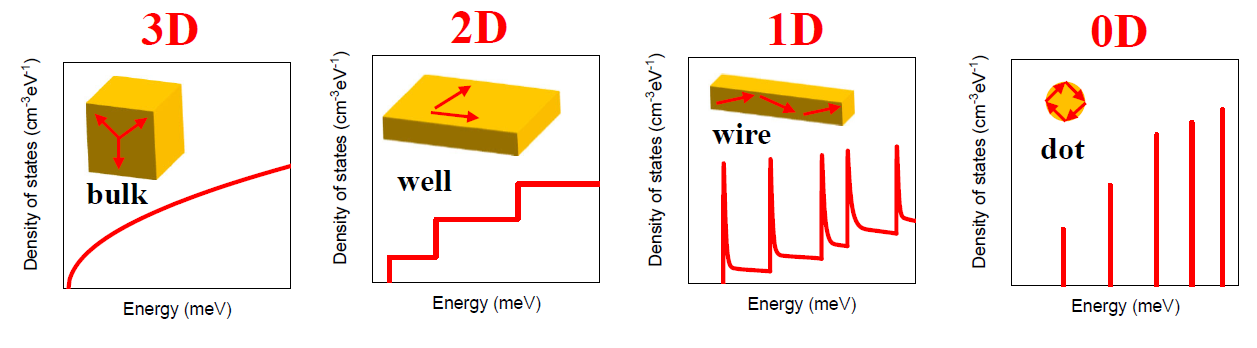
\includegraphics[width=\linewidth]{img1.png}
    \caption{Schematic of low-dimensional semiconductor structures and the schema of energy level, with respect to the density of states $D(E)$. Taken from \cite{WarwickSemiconductorsGroup2025}.}
\end{figure}

\begin{quote}
    Continuing advances in MBE and breakthroughs in nanolithography has made it possible to confine the electrons; further in more dimensions which leads to quasi-one and quasi-zero dimensional semiconductor structure. Quasi-zero dimensional structures behave like artificial atoms. For example quasi-one-dimensional MOSFET in silicon have revealed the universal conductance fluctuations due to random quantum interference predicted by Altshuler et al. \cite{Peeters1992LowDS}.
\end{quote}
He also emphasized that the essentiality of low-dimensional systems is their particular density of states. The latter in which was mentioned, is "the number of available electron states per unit energy", all of which links to the properties of transport and confinement protocols.

\subsection{Structural commitments}
When moving from textbook wells to realistic condensed-matter heterostructures, several modelling approximations and their domains of validity become critical, especially considering physical realization of such. First, is the assumption on non-interacting electron inside confinement. Such is to say, we neglect electron-electron correlation and excitonic binding unless explicitly included in the model. This basically gives us formulaic strength - to solve a many-body system of well-behaved independency, we can solve only the system of Schrödinger equation with single-particle formulation, thus staying in the zone of the first quantization effectively. The method works practically well as an \textit{approximate simplification} condition for various cases, and is a requirement for the working of the free electron model, nearly-free electron model, alongside Bloch's theorem for crystals lattice, as seen in literature \cite{Fulde1995,McGuire_1997}. However, in region where this assumption might be the dampening prediction, or where such electron-electron interaction cannot be considered null as for them to be the major mechanism, divergence happens, often strong breakdown, as seen in particular, of the sequential double ionization problem space \cite{Pfeiffer_2011}. 

Second, is the effective-mass approximation (EMA) usage of the carrier electron, thus also $k\cdot p$ expansion. Per historical development, we get a model of Bloch's electron (1929) from Bloch's theorem, in which dynamics in a periodic potential can be expressed in such. In principle, Bloch's wave theorem for specifying electron form, similar to the independent electron approximation, assumes that such many-electron interaction is lumped together into an effective electron potential. Doing such, it dramatically reduces the complexity of the model, and thus having him to solve only the reduced setting for
\begin{equation}
    \begin{split}
        &\hat{H}\psi(\mathbf{r}) = \left(-\frac{\hbar^2}{2m}\nabla^{2} + V(\mathbf{r})\right)\psi(\mathbf{r}) = E\psi(\mathbf{r})\\
        & \Delta \psi + \mu (E-V)\psi = 0, \quad \mu = (8\pi^{2}m)/\hbar^{2}
    \end{split}
\end{equation}
for $V(\mathbf{r})$ is a periodic potential with the lattice periodicity as said before. On the space of three-dimensional system consideration of the crystal, the solution that Bloch reached from his paper \cite{blochUberQuantenmechanikElektronen1929a}, formulated the solution of the wavefunction as
\begin{equation}
    \psi_{klm}(x,y,z) = \exp{\left( 2\pi i \dfrac{kx}{K}+\dfrac{ky}{L}+\dfrac{kz}{M} \right)}u_{klm}(x,y,z)
\end{equation}
More details can be taken from the original paper, or review papers of the original. Per simplification models, as specified of Rabinovitch \cite{PhysRevB.4.1017}, Hyeonwoo et al. \cite{Yeo_2020}, or Donetti et al. \cite{10.1063/1.3639281}, EMA is a very effective, simplified model of Bloch's electron under certain conditions, for both computational and numerical simulation purpose, as well as analytical one for well-behaved system. For a nearly parabolic band near extremum $k_{0}$, the effective mass tensor $m_{ij}^{*}$, energy dispersion $E(\mathbf{k})$, $\mathbf{k}$ being the crystal wavevector can be connected as
\begin{equation}
    \frac{1}{m_{ij}^{*}} = \frac{1}{\hbar^2} \frac{\partial^{2}}{\partial k_{i}\partial k_{j}}E(\mathbf{k}) \Bigg\rvert_{\mathbf{k}=k_{0}}
\end{equation}
However, as they also pointed out, the method can be considered crude approximation in many settings, for example, hole transport, where "strong non-parabolicity and anisotropy of silicon valance band makes EMA a very crude approximation". Alongside envelop function \footnote{The envelope function refers to a mathematical representation of a wavefunction in quantum wells, characterized by a plane wave in the in-plane directions (x, y) and a localized wavefunction in the z-direction, normalized to the sample area. It describes the spatial distribution of particles confined in a quantum system while allowing for extended states in the unconfined directions \cite{EnvelopeFunctionOverview}.} and $k\cdot p$-expansion \cite{Li_2014} (\cite{M_G_Burt_1999} for fundamentals discussion of both conventional and envelop theories for modern semiconductor physics of the time), they form the bulk of theoretical tools for working on slow-varying spatial modulation of the electron, in other word, when the expressed envelop representation varies slowly on the scale of a lattice constant and inter-band mixing is small. As such, it breaks down for also regions with abrupt interfaces, strong strains, or very narrow wells. The representation of envelope function for heterojunctions also introduces boundary conditions that are often unsafe and should be proceeded carefully, and thus requires in certain case, justifications, as seen for microstructures \cite{Burt1992TheJF}. 

Along the way, there are practical assumptions on smoothness, and penetration depth to be enough for quantization. However, with material offset in practice, such as chemical composition, strain, interface states being susceptible to such and also the well depth; and quantum size limits of scaling downward in current semiconductor development, where one can reach extremely small physical thickness between layers, where scattering, disorder and phonons amplifies quantization breakage, and forcing experimental conditions to be high (for example, high quality materials). The most important distinction or rather potential point of confusion, justifiably so, is the conjunction between classical, semi-classical dynamics (in which effective mass on mass tensor is an artefact of), and quantum interpretation intersects of material structures and models. Essentially, we are to admit inconsistency and approximated results, with potential realization that epistemically and ontologically, those models are bundles of non-exact interpretation and patterns, thus requires explicit framing of effectiveness, if not to be unable to trace back on failing points or divergent results when applied of different settings. 


\subsection{Quantum potential topology justification}

So far, we have been discussing the potential intervention from external conditioning, leading to boundary condition and wavefunction energy landscape, and so forth. However, one would also add. It is really relevance, or at least that important in determination of the system? Why should one care, if for example, certain conditioning of the theoretical framework pertains to the idea of symmetry and invariance, such is to say of different potential, it is the same physics, thence implicitly allow for potential injection in the form of solving dynamical equation for $V_{1}(q)$, $V_{3}(q)$, enables solving for $V_{1}(q)+V_{2}(q)$? 

Indeed, such change can happen intuitively, and supposedly the general notion of \textbf{topology} suggests a form of continual buildup. That is, given two potential, the topological landscape should operate, in hindsight, similar to a convolution over the arbitrary potential field, leaving us with feasible linear addition on potential landscape. However, such only works if the potential itself is defined as scalar on the configuration space of the dynamical, be it Schrödinger or Dirac, or von Neumann equation, or Heisenberg picture. They change encoding of the supposed system under configuration, but not the system below it. This is the trade-off of quantum mechanics, and one simple cannot ignore this. 

One example that would make sense, is in the discrepancy between quantum mechanical treatment and classical treatment where the philosophy of specification is different. Ontology in classical physics is absolute; one defines properties of the system, and assigns them as given to objects, following by rules under assumptions of interactions, and so on. As said, we say classical physics is externally enforced, and thus bear the limitation of specification frame. That is also why the topic of symmetry was developed during the onset of theoretical mechanics, as a mechanism toward controlling and confining runaway argument of this classical view, while effective, introduces frame relativity, and framework mismatch artefact. Quantum mechanics, on the other side, notice categorical error, on the frame $Q[P]$ upon the physical world $P$ to be insufficient, and often, misaligned to the physical realization itself. Such prompts the reversal action, where one defines $\Psi$ as the placeholder of all sufficient information given of the system, and must be extracted from interaction, or inference, of which is to say the underlying physics is hidden under a black-box, and can only be extracted. This, trades transparency and the capacity of specification on details, toward probabilistic framing and knowledge objectivity, thus allowing quantum physics to take on physical behaviours much more freely and accurately, because of frame shift. Under the same line of argument, we can also understand why Bell's inequality works against hidden variable conjecture. For the hidden variable conjecture to work, it must assume there exists a frame $Q'\supset Q$ previously, that will explain $Q$. However, this brings about the presumption that $Q'$ is the true state of the world, thus before any success can be taken down, $Q'$ simple cannot beat the other side of Bell's inequality, because the inequality itself is forced from the object itself. Any act of external referencing is inconsistent with the physical oracle being the object encoded for decryption (i.e. quantum results), so to speak. This works against locality and realism, where one can say that they are ontological commitments about how information and causation work, and how state with measurement works, respectively, and thus not strictly the physical reality. In together, they assert that "measurement outcomes reference a pre-existing external state of affairs.", which is \textbf{really strong} of an argument \footnote{In essence, what we say is: classical models assume specification completeness. Quantum mechanics assumes interaction-completeness. And finally, the wavefunction is not a state of reality but a sufficient encoding under epistemic constraint, and that is exactly why it works.}. 

That said, such behaviour is typically hard to erase, and there exists a wide-spread problem, where analytical thinking indeed penetrates and assume such stance of the hidden variable interpretation, or rather to fix ontological completeness. For instance, this affects mainly the \textit{analytical method} (or closure of such), if not done correctly, into assuming hidden variable conjecture by itself. This is because of the formation of though where theorems and formal language takes precedence, and thus locking the interpretation in such frame. Because this is a frame, it is treated as similar to saying the formalism is complete as explanation. Which, by itself, invalidates the presumption of quantum mechanics, and Bell's inequality until invoked. Such is also why damage control is often used for justification of models and approximations, as declared and seen in previous section, where one requires justification to apply EMA, and identifying error regions outside EMA's approximation range. Such is also the position on modeling that we will have in mind. 

Moving on, the hidden consequences of quantum physics by then, indicate that the topology itself is rather not scalar, but, the Hamiltonian that encodes such landscape, is an operator. Hence, the potential itself, is expressing a functional space. Such is why while it is intuitive to think of solving $V(x)$ separately, operator group actions, energy discrete levels, transfer topology, and different system depictions change from first order fixture of the Hamiltonian. Thence, unless each potential remains structurally continuous on functional space, which in certain cases are impossible, especially since they are not spectral composition, we cannot solve them separately without introducing additional scaffolding. This is also a problem, and hedges a question of certain modified Hamiltonian that allows spectral decomposition on linearity requirement of the potential topology. Those are conditions of quantum physics. Thence, while acknowledging it as an effective theory, we work within its set of solution consequence, and would reserver such argument on spectral decomposition in another discourse of modified Hamiltonian and the structural presumption needed for an upgraded configuration space. Notably, during $n$th order configuration space addition, one inherits avoidance of solution pathologies, and structural debt.

\section{1-D Confinement - Quantum Well}

When we apply potential topology on spatial one-dimension, what we get is a \textbf{quantum well}. Functionally, it is a type of constrained system that reduce a system of three-dimensional into a two-dimension free-motion system. The act can be called as dimensional reduction of specific microscopic matter, which is then called \textit{low-dimensional system} for any system that can be expressed as such. This is ultimately used for modelling capture structures of quantum scale, for example, a system of semiconductor (\texttt{GaAs} for example). The quantum well in equation~\ref{eq:quantum_well_main_1} 
\begin{equation}\label{eq:quantum_well_main_1}
    V(z)=\begin{cases}
        V_{0} & z \leq L_{1} \\
        \dfrac{1}{2}m_{{e}}\omega_{z}^{2}z^{2}+  V_{ext}(z) & L_{1} < z < L_{2}\\
        V_{0} & z \geq L_{2}
    \end{cases}
\end{equation}
is one of such quantum well, restricting on the $z$-axis only, leaving the other two dimension free of particle. Often, the form of such quantum well is not trivial, for example, we can see that it has the harmonic terms on the left, and an external quantization $V_{ext}(z)$ to the right. Such $V(z)$ can be used to express certain effects of external, non-fixed potential application from different sources, and so on, of which are particularly interesting. 

For a starter non-trivial case, let us analyse a complex well, best described as a semi-parabolic, finite asymmetric \textit{non-additive} quantum well. It will also aid us partially in the procedure typically employed to solve this kind of behaviour from the potential topology. Thus, consider a one-dimensional potential along the $z$-direction given by:
\begin{equation}
    V(z) = 
\begin{cases}
V_0, & z < 0 \\
\dfrac{1}{2} m_e \omega_z^2 z^2, & 0 \le z \le L \\
V_0, & z > L
\end{cases}
\end{equation}
for $m_{e}$ the effective mass of the electron, $\omega_{z}$ as the confinement frequency, and $U_0 = \frac{1}{2} m_e \omega_z^2 L^2$ is the barrier height, with $L$ the well width. Asymmetry arises from the cutoff at $z=0$ of the semi-parabolic critical shape, while non-additive is referring to the absence of the term
\begin{equation}
    \dfrac{\hbar^{2}\beta_{z}}{2m_{e}z^{2}}
\end{equation}
of which is often called the \textbf{$1/z^2$ effective potential}, or inverse-square, centrifugal potential. In our earlier example potential, $V_{ext}(z)$ can also include such term, however when it is included, often the potential well would be explicit about such choice. The topic is rather well-studied, with mathematical analysis presented for both square potential \cite{Ishida_2025} and inverse-square rigorous proofs in literature \cite{chorfi2024uniquenessschrodingerequationinverse}. The reason for the existence of this term, is usually related to, the system consideration, for example, in heterostructures, curved interfaces, or strongly confined direction. Coordinate transformation and envelop-function reduction thus encode such boundary conditions on $\beta_{z}$, and the overall structure of the expression with molecular interactions. That said, in our case, we do not include such term in, while in practice much structure might have at least partially similar potential shape. 
Since the original system of consideration is three-dimensional, a way to separate such well is to consider the three-dimensional Schrödinger equation,
\begin{equation}
    \begin{split}
        E \Psi(x, y, z) &= -\frac{\hbar^2}{2m_e} \left( \frac{\partial^2 \Psi}{\partial x^2} + \frac{\partial^2 \Psi}{\partial y^2} 
         + \frac{\partial^2 \Psi}{\partial z^2} \right) \\
         &\quad + V(x, y, z) \Psi(x, y, z) 
    \end{split}
\end{equation}
Given that the potential depends only on $z$, we can theorize the separation into as: 
\begin{equation}
  \Psi(x,y,z)=\psi_{\perp}(\vec{r}_{\perp})\psi_{n}(\vec{r})\varphi(t), \quad \vec{r} = (x,y,z)
\end{equation}
Where $\psi_{\perp}(\vec{r}_{\perp})$ is the wavefunction of the waveform along the non-restricted, free space of the $Oxy$ plane, while $\psi_{n}(\vec{r})$ is the restricted waveform along the $z$ axis. In resultant, we gain two expressions of the quantum well aside from time-dependent functional. For the reduction of notation, denoting $\psi(x,y)$ as the free plane wavefunction and $\psi(z)$ corresponding to the well dimension, we first have the free plane $\mathrm{Oxy}$, in which the Schrödinger equation reads with no potential,
\begin{equation}
  -\frac{\hbar^{2}}{2m_e} \left(\frac{\partial^{2}\psi(x,y)}{\partial x^{2}}+\frac{\partial^{2}\psi(x,y)}{\partial y^{2}}\right)  = E_{\perp}\psi(x,y),
\end{equation}
for $U(x,y)=0$. We can solve this as normal within assumption of separable solutions to singular $x$-equation and $y$-equation, and thus leading to the consideration of the well in the free-space. For the $z$ restricted axis, we have the Schrödinger equation,
\begin{equation*}
  -\frac{\hbar^{2}}{2m_e}\left(\frac{\partial^{2}\psi(x,y,z)}{\partial z^{2}}\right)+V(z)\psi(z)=E_{z}\psi(z),
\end{equation*}
or rewriting it in an explicit way,
\begin{equation}
  -\frac{\hbar^{2}}{2m_e}\left(\frac{\partial^{2}\psi(x,y,z)}{\partial z^{2}}\right)+\left( \frac{1}{2}m_{e}\omega_{z}^{2}z^{2} \right)\psi(z)=E_{z}\psi(z)
\end{equation}
for the region $0 < z < L$ Inside the well. Within this setup, we can now proceed with solving it by the normal regional analysis on boundary conditions. We note that at here, the boundary conditions are not optional. For finite barrier on semi-parabolic well, $\psi$ is often considered to be continuous at $z=0$ and $z=L$ per normal quantum potential usage (see \cite{griffiths2018,sakurai2017} and textbook materials \cite{davies1998} for this), alongside, if required, $C^{2}$-differentiable condition on differential operators. Outside such well, the solutions are \textbf{exponentially decaying} due of the physical interpretation of the quantum well. Per specification basis, we consider quantum tunnelling negligible and focus on penetration depth guarantee, as well as confinement region. 
\subsection{Outer well ($z<0$, $z>L$)}
Since in this region, $E_{z}<V_{0}$, the time-independent Schrödinger equation gives decaying or exponentially damped solution in both barrier, assuming infinite barrier depth, 
\begin{equation}
    -\frac{\hbar^2}{2m_e} \frac{d^2}{dz^2} + (V_{0}-E_{z}) = 0,
\end{equation}
which gives
\begin{equation}
    \psi \propto \exp{(\pm \kappa z)}, \quad \kappa = \sqrt{\dfrac{2m(V_{0}-E_{z})}{\hbar^2}}
\end{equation}
The solution is generic, and for physically acceptable bound states, we keep only the decaying exponential, such that
\begin{equation}
    \psi(z<0) \propto \exp{(+\kappa z)}, \quad \psi(z>L) \propto \exp{(-\kappa[z-L])}
\end{equation}
respectively. This is for the presumption of directional penetration from both side of the barrier wall. 
\subsection{Inner well ($0 < z < L$)}
Here, the equation becomes
\begin{equation}
    \left[ -\frac{\hbar^2}{2m_e} \frac{d^2}{dz^2} + \frac{1}{2} m_e \omega_z^2 z^2 \right] \psi(z) = E_{z} \psi(z)
\end{equation}
Thus it is the equation of a one-dimensional harmonic oscillator, but with asymmetric domain, and with solutions given by parabolic cylinder functions due to the truncated domain. We can solve it using the normal way, on bound states since the well is not much different than the typical parabolic form, with different boundary solution only. Or, another way is to do it of \textit{quantum kinematic}, and non-dimensionalize the wavefunction as well. Nondimensionalization in this case can often be considered a move to reduce dimensional dependence, on energy scales or dimensionality mismatch, and let us work more on the parameter dependency tracking purpose, as well as making it cleaner to observe boundary-induced effect. We would like to explore this method, or the interpretation of this way, for that reason. Multiply both sides of the equation by $\dfrac{2}{\hbar \omega_z}$ gives
\begin{equation}
    \left[ \frac{-\hbar}{m_e \omega_z} \frac{d^2}{dz^2} + \frac{m_e \omega_z z^2}{\hbar} \right] \psi(z) = \frac{2E_{z}}{\hbar \omega_z} \psi(z),
\end{equation}
For the dimensionalization constant, set  $\alpha_z = \sqrt{\hbar /m_e \omega_z}$ and $ \delta = z/\alpha_{z}$, we transform the equation into 
\begin{equation}
    \left[ -\frac{d^2}{d\delta^2} + \delta^2 \right] \psi(\delta) = \frac{2E_{z}}{\hbar \omega_z} \psi(\delta)
\end{equation}
or rather can be written with factorization as
\begin{equation}
    \Rightarrow \psi''(\delta) + \left( \frac{2E}{\hbar \omega_z} - \delta^2 \right) \psi(\delta) = 0
\end{equation}
To solve this, we assume the solution to have the form similar to $\psi(\delta) \sim u(\delta) e^{-\frac{\delta^2}{2}}$ without fixture. There, the equation turns into
\begin{equation}
    \left[ u''(\delta) - 2 \delta u'(\delta) + \left( \frac{2E}{\hbar \omega_z} - 1 \right) u(\delta) \right] e^{-\frac{\delta^2}{2}} = 0
\end{equation}
which can be simplified into the Hermite differential equation, depending on the analysis. From simple analysis, we see that this is the equation of the harmonic oscillator, and the solutions are Hermite polynomials multiplied by a Gaussian, with discrete energy levels:
\begin{equation}
    E_n = \hbar \omega_z \left(n + \frac{1}{2}\right)
\end{equation}
By normalizing and transforming the equation into the one-dimensional harmonic oscillator form, we determine the discrete energy spectrum and the asymptotic wavefunction shape in the parabolic region $0 < z < L$. Simplifying the equation,
\begin{equation}
    u''(\delta) - 2\delta u'(\delta) + u(\delta) \left[ \frac{2E}{\hbar \omega_z} - 1 \right] = 0
\end{equation}
From here, we let $\lambda = 2E/\hbar \omega_z - 1$, the equation then becomes
\begin{equation}
    u''(\delta) - 2\delta u'(\delta) + \lambda u(\delta) = 0
\end{equation}
Noticeably, this is the Hermite differential equation with condition $\lambda = 2N$. Upon such realization, therefore, we have
\begin{align}
    &u(\delta) = H_N(\delta)\\
    &\psi(\delta) \sim u(\delta) e^{-\delta^2/2} = H_N(\delta) e^{-\delta^2/2}
\end{align}
thus giving us the solution in the form
\begin{equation}
    \psi(\delta) = A e^{-\delta^2/2} H_N(\delta)
\end{equation}
with
\begin{equation}
    \delta = \frac{z}{\alpha_z}, \quad \alpha_z = \sqrt{\frac{\hbar}{m_e \omega_z}}
\end{equation}
The final wavefunction in terms of $z$ can then be written as
\begin{equation}
    \psi(z)= A \exp\left(-\frac{z^2}{2\alpha_z^2}\right) H_N\left(\frac{z}{\alpha_z}\right)
\end{equation}
leaving us with the only requirement now to analyse boundary condition, and apply normalization. At $z=0$, $\psi(0)=(0) = A H_N(0)$, and so is for $z=L$ as a precondition on equal wall well. Depending on the boundary condition (e.g., infinite potential wall or symmetry/asymmetry), we choose appropriate $N$ values (even or odd). Wavefunction normalization for $N=0$ or $N=1$ gives solving
\begin{equation}
    \int_0^L A_N^2 \exp\left(-\frac{z^2}{\alpha_z^2}\right) H_{N+1}^2\left( \frac{z}{\alpha_z} \right) dz = 1
\end{equation}
such that, for $N=1$,
\begin{equation}
    A_0 = \left[ -2 e^{-\frac{L^2}{\alpha_z^2}} \cdot L + \alpha_z \sqrt{\pi} \, \mathsf{Erf}\left( \frac{L}{\alpha_z} \right) \right]^{-\frac{1}{2}}
\end{equation}
for $\mathsf{Erf}$ the asymptotic error function associated. For $N=1$,
\begin{equation}
    A_1 = \left[ \frac{16 e^{-\frac{L^2}{\alpha_z^2}} \cdot L \cdot J}{\alpha_z^4}
+ 24 \alpha_z \sqrt{\pi} \, \text{Erf}\left( \frac{L}{\alpha_z} \right) \right]^{-\frac{1}{2}}
\end{equation}
for $J=-3 \alpha_z^4 + \alpha_z^2 L^2 - 2 L^4$, and complete the wavefunction analysis of this particular potential well. For the well alone, it has rather nontrivial but deliberate application of the field. More specifically, for example, in analysis of quantum well field-effect transistor, The input voltage induces an asymmetric potential along the channel, which can be modelled using a semi-parabolic well to optimize carrier current. In semiconductor lasers and IR emitters, quantum energy level spacing determines emission wavelength; adjusting $\omega$ and $L$ helps fine-tune the spectrum and thus a fairly accurate approximation, and so on. 


%%%%%%%%%%%%%%%%%%%%%%%%%%%%%%%%%%%%%%%%%%%%%%%%%%%%%%%%%%%%%%%%%%%%%%%%%%%%


\section{Nonlinear absorption in complex well}

Our quantum system in consideration of this section is of the form: 
\begin{equation}\label{eq:quantum_well_main_3}
    V(z)=\begin{cases}
        V_{0} & x \leq L_{1} \\
        \dfrac{1}{2}m_{{e}}\omega_{z}^{2}z^{2}+ \dfrac{\hbar^{2}\beta_{z}}{2m_{e}z^{2}} + V_{ext}(z) & L_{1} < x < L_{2}\\
        V_{0} & x \geq L_{2}
    \end{cases}
\end{equation}
Where $\omega_{z}$ is the angular momenta of the electron in the $z$-direction, $m_{e}$ the rest mass, $\hbar$ as Planck reduced constant, $\beta_{z}$ is the intrinsic constant of the quantum well configuration, and $V_{ext}(z)$ the external electric field of uniform polarized strength in the same dimension. The goal of the main research is then to analyse the nonlinear absorption coefficient of strong electromagnetic waves for electrons confined in an asymmetric finite semi-parabolic quantum well with resonance in the presence of electric fields. Of such, successive operations and formulation will be extensively expressed. 

In our above well, we notice that it models the factors: 
\begin{equation}
    V_{1}(z)=\frac{1}{2} m_{{e}}\omega_{z}^{2}z^{2},\quad V_{2}(z)=\frac{\hbar^{2}\beta_{z}}{2m_{e}z^{2}},\quad V_{3}(z) = V_{ext}(z)
\end{equation}
where $V_{1}$ is the half-parabolic (by the coordinate of the range $[L_{1},L_{2}]$), antisymmetric potential, which model a saddle point of potential (simulating some imperfect electron-pulling region), $V_{2}$ simulates the smoothing version of the normal square well, by adding reduction on the scale of inverse-square law (factor $1/z^{2}$), and $V_{3}$ for external field potential. 
\subsection{Quantum well without external field}
For equation~\ref{eq:quantum_well_main_3}, its energy spectrum can be calculated for the external electrical field. If such external field is ruled out, so $V_{\mathrm{ext}}(z)=0$, then 
\begin{equation}\label{eq:quantum_well_main_2}
    V(z)=\frac{1}{2}m_{{e}}\omega_{z}^{2}z^{2}+ \frac{\hbar^{2}\beta_{z}}{2m_{e}z^{2}} 
\end{equation}
The Schrödinger equation for time-independent, assuming separable solution as always is then:
\begin{equation}
    -\frac{\hbar^{2}}{2m_{e}} \frac{\partial^{2}}{\partial z^{2}} \phi_{n}(z) + V(z)\phi_{n}(z) = E\phi_{n}(z)
\end{equation}
which is written as we change to the final state of $V(z)$:
\begin{equation}
    -\frac{\hbar^{2}}{2m_{e}} \frac{\partial^{2}}{\partial z^{2}} \phi_{n}(z) + \left[\frac{1}{2}m_{{e}}\omega_{z}^{2}z^{2}+ \frac{\hbar^{2}\beta_{z}}{2m_{e}z^{2}}\right]\phi_{n}(z) = E\phi_{n}(z)
\end{equation}
This equation is reserved for the $z$-axis, every other axis can be resolved using the free-particle case. The solution to such problem gives the wavefunction: 
\begin{equation}
    \phi_{n}(z) = A_{n}z^{2s}\exp{\left(-\frac{z^{2}}{2\alpha_{z}^{2}}\right)}L^{\delta}_{n}\left(\frac{z^{2}}{\alpha_{z}^{2}}\right)
\end{equation}
where $L^{\delta}_{n}$ are Legendre polynomials, with the following constants: 
\begin{equation}
    s=\frac{1}{4}\left(1+\sqrt{1+4\beta_{z}}\right), \quad \delta = 2s - \frac{1}{2}, \alpha_{z} = \sqrt{\frac{\hbar}{m_{e}\omega_{z}}}
\end{equation}
Here, the constant $A_{0}$ is just the normalization constant. Hence, it must satisfy: 
\begin{equation}
    A_{n}^{2} \int_{0}^{L} \left[z^{2s}\exp{\left(-\frac{z^{2}}{2\alpha_{z}^{2}}\right)}L^{\delta}_{n}\left(\frac{z^{2}}{\alpha_{z}^{2}}\right)\right]^{2} \: dz = 1
\end{equation}

The ground and first initial state of this wavefunction is 
\begin{align}
    \phi_{0}(z) & = A_{0}z^{2s}\exp{\left(-\frac{z^{2}}{2\alpha^{2}_{z}}\right)} \\
    \phi_{1}(z) & = A_{1} z^{2s}\exp{\left( -\frac{z^{2}}{2\alpha^{2}_{z}} \right)} \left(-\frac{z^{2}}{\alpha_{z}^{2}}+\gamma + 1\right)
\end{align}
which has normalization constant using such calculation being 

\begin{align}
    A_{0} & = \sqrt{2}\alpha_{z}^{-1/2-2s} \left[\Gamma \left(\frac{1}{2}+2s\right)\Gamma\left(\frac{1}{2}+2s, \frac{L^{2}}{\alpha_{z}^{2}}\right)\right]^{-1/2}\\
\end{align}
and 
\begin{equation}
    \begin{split}
        A_{1} & = 2\sqrt{2} \alpha_{z}^{-1/2-2s} \\
    & \times \Big\{ \Big[3+4\gamma^{2}+\gamma(4-16s)+16s^{2}\Big] \\
    &\quad \quad  \Gamma\left(\frac{1}{2}+2s\right)- T_{1} - T_{2}\Big\}
    \end{split}
\end{equation}
for the two terms $T_{1},T_{2}$ being
\begin{equation}
    T_{1} = 4(1+\gamma)^{2} \Gamma\left(\frac{1}{2}+2s, \frac{L^{2}}{\alpha_{z}^{2}}\right) + \gamma(1+\gamma) \Gamma \left(\frac{3}{2}+2s, \frac{L^{2}}{\alpha_{z}^{2}}\right)
\end{equation}
and 
\begin{equation}
    T_{2} = 4\Gamma \left(\frac{3}{2}+2s, \frac{L^{2}}{\alpha_{z}^{2}} \right)
\end{equation}

The energy spectrum of the quantum well is then calculated as 
\begin{equation}
    \mathcal{E} = \hbar \omega_{z} \left( 2n+1 + \frac{1}{2}\sqrt{1+4\beta_{z}} \right)
\end{equation}
which reduces to $\hbar\omega_{z}(2n+3/2)$ when $\beta_{z}\to 0$. In general, the form constant is calculated of 
\begin{equation}
    I_{z} = 2\int \phi^{*}_{0}(z)\cos{(q_{z})z}\phi_{1}\:dz, \quad I_{q_{z}} = \int_{-\infty}^{+\infty} \lvert I_{z}\rvert^{2} \: dq_{z}
\end{equation}
\subsection{With electric and magnetic field}

In the case of perpendicular within radial axis of electrical field $\vec{B}(0,0,B)$ and magnetic field $\mathbf{E}(E,0,0)$, we can solve it `totally similar' to the case of semi-parabolic, asymmetric infinite well, hence the form of the wavefunction is still
\begin{equation} 
    \phi(\vec{r}) = \phi_{0}\Phi(x-x_0)\exp{(ik_{y}y)}\phi_{n}(z)
\end{equation}
where $\Phi(x-x_0)$ is the harmonic wavefunction centres at $x_{0}$, $\phi_{n}(x)$ the calculated step wavefunction, for \begin{equation}
    x_{0} = -\frac{\hbar}{eB} \left( k_{y} + \frac{m_{e}E}{\hbar B} \right) = \ell^{2} \left(k_y - \frac{m_e v_{d}}{\hbar}\right)
\end{equation}
The energy spectrum does not change much, 
\begin{equation}
    \begin{split}
        \mathcal{E} &= \hbar \omega_{z} \left( 2n+1 + \frac{1}{2}\sqrt{1+4\beta_{z}} \right) \\
        & \quad + \left(N+\frac{1}{2}\right)\hbar \omega_{c} + \hbar v_{d} k_{y} - \frac{1}{2} m_{e}v_{d}^{2}
    \end{split}
\end{equation}
thus we would be considering a well-observed bracket of solution. 
\subsection{Nonlinear absorption with electromagnetic waves}

To start with the analysis, we need some formulations of the interaction of electron, phonon and external electrical field within the confinement of the quantum well. This can be separated to three operators interactions: external electric field interaction, non-interacting phonon interaction, and electron-phonon interaction. 

Call $z$ the space spatial axis being quantized, the Hamiltonian for the electromagnetic-phonon interaction in the quantum well when there exists external electric field $\mathbf{E}(t)=\mathbf{E}_{0}\sin{(\Omega t)}$ as the following separation expression of interacting terms:
\begin{align}
    &\mathcal{H}\\
    & = \underbrace{\sum_{n,\vec{k}_{\perp}} \mathcal{E}_{n}\left(\vec{k}_{\perp} - \frac{e}{\hbar c} \vec{A}(t)\right)a^{+}_{n,\vec{k}_{\perp}} a_{n,\vec{k}_{\perp}} }_{\text{external field}} \\ 
    & \underbrace{\quad + \sum_{\vec{q}} \hbar \omega_{0} b_{\vec{q}}^{+} b_{\vec{q}}}_{\text{non-interacting phonons} } \\
    & \underbrace{\quad + \sum_{\vec{q}} \sum_{n,n', \vec{k}_{\perp}} C_{\vec{q}} I_{n,n'}(q_{z}) a^{+}_{n',\vec{k}_{\perp}+\vec{q}} a_{n,\vec{k}_{\perp}} \left(b_{\vec{q}} + b^{+}_{- \vec{q}}\right)}_{\text{electron-phonon }}
\end{align}
with $\mathcal{E}_{n}$ is the energy of the electron, $\vec{k}_{\perp}, \vec{q}$ are the vectors of electron and phonon in the system respectively, $\ket{n; \vec{k}_{\perp}}$, $\bra{n;\vec{k}_{\perp}+\vec{q}}$ being the system's electron state before and after the scattering interaction of the system. For the external field, which is considered orthogonal, $\vec{A}(t)$ is expressed as the electrical potential 
\begin{equation}
    -\frac{1}{c} \frac{d}{dt} \vec{A}(t) = \mathbf{E}_{0}\sin{(\Omega t)},\quad  \vec{A}(t) = \frac{c}{r} \mathbf{E}_{0}\cos{(\omega t )}
\end{equation}
$I_{n,n'}(q_{z})$ is the electronic form factor of the heterogenous, constituent superlattice - in our case of quantum well is a special case. This is usually expressed as 
\begin{equation}
    \begin{split}
        &I_{n,n'}(q_{z}) \int_{0}^{N_{d}} \Psi^{*}_{n}(z) \Psi_{n'}(z)\exp{(iq_{z}z)}\: dz \\
        &= \frac{2}{L} \int_{0}^{L} \Psi^{*}_{n}(z)\Psi_{n'}(z)\exp{(iq_{z}z)}\: dz
    \end{split}
\end{equation}
in which $2/L$ is the intrinsic normalization factor for the special case of a quantum well. Energy spectrum $\mathcal{E}_{n}(\vec{k}_{\perp})$ here is expressed by 
\begin{equation}
    \begin{split}
        \mathcal{E}_{n}(\vec{k}_{\perp}) &= \frac{\hbar^{2}}{2m^{*}} \left( k_{\perp}^{2} + k_{z}^{n^{2}} \right) \\
        &= \hbar \Omega_{B} \left(N + \frac{1}{2}\right) + \left(\frac{\hbar^{2}}{2m^{*}} \frac{\pi^{2}n^{2}}{L^{2}}\right)
    \end{split}
\end{equation}
where $\Omega_{B}=(eB)/(m^{*}c)$ is the cyclotron frequency of the external field. 

Finally, before jumping into the section of the quantum effect and motions for the system, given the above Hamiltonian, we will use the following commutative operator between the observable operators in the Hamiltonian, such as the following: 
\begin{align}
     [a_{i} ; a_{k}^{+}]  &= a_{i}a_{k}^{+} + a^{+}_{k}a_{i} = \delta_{ik} \\
    [a_{i}^{+} ; a_{k}^{+}] & = \{ a_{i}; a_{k} \} = 0 \\
    [b_{i} , b_{k}^{+}] & = b_{i}b^{+}_{k} - b_{k}^{+}b_{i} = \delta_{ik} \\
    [b_{i}^{+}; b_{k}^{+}] &= \{b_{i} ; b_{k}\} = 0
\end{align}
Those will be our tools for the momentum expansion in later section. 
\subsection{The momentum operator}
In nonlinear absorption, the observable set is the current, momentum, and polarisation. Such is the reason why we would like to solve the momentum operator, which further use and interaction of such in the quantum well as well as constructing quantum-mechanical expression hedge the usage of the momentum operator expression for \textbf{particle number operator}. We have the following expression as baseline for such, 
\begin{align}
    i \hbar \frac{\partial f_{n, k_{\perp}}(t)}{\partial t} = \left\langle \left[ a^{+}_{n,\vec{k}_{\perp}}  a_{n,\vec{k}_{\perp}}; H \right] \right\rangle,
\end{align}
with
\begin{equation}
    f_{n, k_{\perp}} = \left\langle a^{+}_{n,\vec{k}_{\perp}} ; a_{n,\vec{k}_{\perp}} \right\rangle.
\end{equation}
We would like to denote the three terms separation above into $H_{2}$, $H_{2}$ and $H_{3}$ for clarification. Applying this for the first term (external force interaction), denoting $S_{1}$, gives us 
\begin{equation}
    S_{1} = \sum_{n,\vec{k}_{\perp}} \mathcal{E}_{n}\left(\vec{k}_{\perp} - \frac{e}{\hbar c} \vec{A}(t)\right)\left[ a^{+}_{n,\vec{k}_{\perp}}  a_{n,\vec{k}_{\perp}}; a^{+}_{n,\vec{k}_{\perp}} a_{n,\vec{k}_{\perp}} \right]
\end{equation}
The commutator in question can be expanded by the commutative identity
\begin{equation}
    \begin{split}
        &\left[ a^{+}_{n,\vec{k}_{\perp}}  a_{n,\vec{k}_{\perp}}; a^{+}_{n,\vec{k}_{\perp}} a_{n,\vec{k}_{\perp}} \right] \\
        &= a^{+}_{n,\vec{k}_{\perp}} a_{n,\vec{k}'_{\perp}} \delta_{\vec{k}_{\perp},\vec{k}'_{\perp}} - a^{+}_{n,\vec{k}'_{\perp}} a_{n,\vec{k}_{\perp}} \delta_{\vec{k}'_{\perp},\vec{k}_{\perp}}
    \end{split}
\end{equation}
Thus admittedly, gives $S_{1}=0$ as a result. Similarly, for the second term on non-interacting phonons, denoted as $S_{2}$,
\begin{equation}
    \begin{split}
        S_{2} & = \left[ a^{+}_{n,\vec{k}_{\perp}}a_{n,\vec{k}_{\perp}} ; \sum_{\vec{q}} \hbar \omega_{\vec{q}} b^{+}_{\vec{q}}b_{\vec{q}} \right] \\
    & = \hbar \sum_{\vec{q}} \omega_{\vec{q}} \left[ a^{+}_{n,\vec{k}_{\perp}} a_{n,\vec{k}_{\perp}}; b^{+}_{\vec{q}}b_{\vec{q}} \right] \\
    & = 0
    \end{split}
\end{equation}
The third term can now be in consideration. Calculation shows that $S_{3}$ can be given in the form
\begin{equation}
    \begin{split}
        S_3 &= \sum_{q_\bot} \sum_{\vec{k'_\bot},\vec{q}}C\left(\vec{q}\right) I_{n,n'} \left(q_z\right) \\
        &\times \left[\left(a^+_{n, \vec{k_\bot}}a_{n',\vec{k_\bot} - \vec{q_1}}b_{\vec{q}}\right)+ \left(a^+_{n', \vec{k_\bot}-\vec{q_1}}a_{n, \vec{k_\bot}}b_{-\vec{q}}\right)^* \right] \\
    & - \left[\left(a^+_{n', \vec{k_\bot}+\vec{q}}a_{n, \vec{k_\bot}}b_{\vec{q}}\right)- \left(a^+_{n, \vec{k_\bot}}a_{n', \vec{k_\bot}+ \vec{q_1}}b_{-\vec{q}}\right)^*\right]
    \end{split}
\end{equation}
From such, as we have seen, the contribution to momentum operator now lies only in this term, and hence, it can be considered the most important term, as expected of the treatment. Returning to the expression, then, we reduce it simply to 
\begin{equation}
    i \hbar \frac{\partial f_{n, k_{\perp}}(t)}{\partial t} = \left\langle S_{3} \right\rangle
\end{equation}
By linearity of the commutator. Here, we introduce a concept, the time-dependent correlation function $F_{n, \vec{k_{1\bot}}, n',\vec{k_{2\bot}},\vec{q'}}(t)$, which describes the expectation value of the following process: we create a particle in state $n,k_{1\bot}$, annihilate one in state $n', k_{2\bot}$, and absorb a phonon with momentum $q'$. This quantity will allow us to rewrite the equation of motion in a more compact form. For now, however, we have  $F_{n,\vec{k_{1\bot}},n', \vec{k_{2\bot}},\vec{q'}}(t)$, which in this case is given by
\begin{equation}
    F_{n,\vec{k_{1\bot}},n', \vec{k_{2\bot}},\vec{q'}}(t) = \left\langle a^+_{n, \vec{k_{1\bot}}}a_{n',\vec{k_2\bot}} b_{\vec{q'}}\right\rangle(t)
\end{equation}
thus having the commutator result of $S_{3}$ to be in the form
\begin{equation}
    \begin{split}
        & \left\langle \left[a^+_{n, \vec{k_\bot}}a_{n,\vec{k_\bot}}, H_{3}\right]\right\rangle  = -\sum_{q'} C\left(\vec{q}\right)I_{nn'}\left(q_z\right) \mathcal{F} ,
    \end{split}
\end{equation}
where $\mathcal{F}$ is defined as
\begin{equation}
    \begin{split}
        \mathcal{F}&=F_{n',\vec{k_\bot}+\vec{q_1},n,\vec{k_\bot,}\vec{q}}\\
        &\quad +F^*_{n,\vec{k_\bot},n',\vec{k_\bot}-\vec{q},\vec{q}}\\
        &\quad -F^*_{n',\vec{k_\bot}-\vec{q},n,\vec{k_\bot},-\vec{q}}
    \end{split}
\end{equation}
Combining the sum of three terms and the functional, we get
\begin{equation}
     i \hbar \frac{\partial f_{n, k_{\perp}}(t)}{\partial t} = -\sum_{q'} C\left(\vec{q}\right)I_{nn'}\left(q_z\right) \mathcal{F}
\end{equation}
or rearranging, gives
\begin{equation}
     \dfrac{\partial f_{n, \vec{k_\bot}}(t)}{\partial t} = -\dfrac{i}{\hbar}\sum_{q'} C\left(\vec{q}\right)I_{nn'}\left(q_z\right) \mathcal{F}
\end{equation}
\subsection{Correlation function}
The correlation function is a natural step from the momentum expression, and we would reserve a section to solve it. The role of the function comes from the nonlinear absorption effect itself. As explained, it encodes the time-dependent expectation value current of the process of absorption. The absorption event specified is composite, and no one-body expectation value can decode that. Hence, we are required to treat them explicitly. Specially more, all microscopic physics have been pushed into the correlation function $\mathcal{F}$, and we switch into population dynamics, which is what we would be doing here. Recall the formulation itself, which gives
\begin{equation}
    F_{n, \vec{k_{1\bot}}, n',\vec{k_{2\bot}},\vec{q'}}(t)= \left\langle a^+_{n,\vec{k_{1\bot}}},a_{n', \vec{k_{2\bot}}}b_{\vec{q}} \right\rangle t
\end{equation}
This is the minimal correlator of the multiple-subsystem dynamics, to express electron state change, phonon participation, and still can be time-resolved by the expression itself. Differentiate on $F$ of the left-hand-side on the momentum equation, we have
\begin{align*}
    i \dfrac{\partial F}{\partial t} &= i \dfrac{\partial}{\partial t}\left(a^+_{n, \vec{k_\bot}}, a_{n', \vec{k_{2\bot}}}b_{\vec{q}}(t)\right)\\
    &= \langle [F,H] \rangle t\\
    &= \left\langle\left[a^+_{n,\vec{k_{1\bot}}},a_{n', \vec{k_{2\bot}}}b_{\vec{q}},H\right] \right\rangle t
\end{align*}
by Heisenberg equation of motion on commutator of the Hamiltonian. First contribution to the commutator, denoted $S_1$, arises from the single particle part, external field of the Hamiltonian. The reason why we are recomputing the supposed zero-contribution parts, is because momentum can evaluate to zero at observable levels, but must be recomputed at correlator level because of the operation of population dynamics. Explicitly, it can be written as followed,
\begin{align*}
    F_1 &= \left \langle \left[a^+_{n,\vec{k_{1\bot}}}a_{n',\vec{k_{2\bot}}}b_{\vec{q'}}, H\right] \right \rangle \\
    &= \sum_{n,\vec{k_{3\bot}}}\mathcal{E}_{n}\left(\vec{k_{3\bot}}-\dfrac{e}{\hbar c}A(t)\right) \mathcal{C}  \\
\end{align*}
for 
\begin{equation}
    \mathcal{C} = \left[a^+_{n,\vec{k_{1\bot}}}a_{n',\vec{k_{2\bot}}}b_{\vec{q'}},a^+_{n,\vec{k_{3\bot}}}a_{n,\vec{k_{3\bot}}} \right]
\end{equation}
Specifically calculating the commutator gives
\begin{equation}
    \begin{split}
        \mathcal{C}
        &= a^+_{n,\vec{k_{1\bot}}} a_{n, \vec{k_{3\bot}}}b_{\vec{q'}}\delta_{n',n, \vec{k_{2\bot}}, \vec{k_{3\bot}}}\\
        &\quad - a^+_{n, \vec{k_{3\bot}}}a_{n', \vec{k_{2\bot}}}b_{\vec{q'}} \delta_{n, \vec{k_{3\bot}}, \vec{k_{1\bot}}}
    \end{split}
\end{equation}
Using the computed commutator, we evaluate $\mathbf{F}_{1}$ again,
\begin{equation}
    \begin{split}
        \mathbf{F}_{1} 
        & = \mathcal{E}_{n',\vec{k_{2\bot}}}\left(\vec{k_{2\bot}}-\dfrac{e}{\hbar c}A(t)\right)\\
        & \quad -\mathcal{E}_{n, \vec{k_{1\bot}}}\left(\vec{k_{1\bot}}-\dfrac{e}{\hbar c}A(t)\right)\left \langle a^+_{n, \vec{k_{1\bot}}}a_{n',\vec{k_{2\bot}}k\vec{q'}}\right \rangle t
    \end{split}
\end{equation}
which itself is irreducible to zero-valued, and thus is the reason why we are required to compute it again. Moving on to $F_{2}$ of the phonon interaction channel, we get
\begin{equation}
    \mathbf{F}_{2} = \left \langle \left[a^+_{n,\vec{k_{1\bot}}}a_{n',\vec{k_{2\bot}}}b_{\vec{q'}}, \sum_{q_\bot} \hbar \omega_{\vec{q_1}} b^+_{\vec{q_1}} b_{\vec{q_1}}\right] \right \rangle
\end{equation}
which gives
\begin{equation}
    \mathbf{F}_{2} =  \hbar \omega_{q'} \left \langle a^+_{n, \vec{k_{1\bot}}}a_{n', \vec{k_{2\bot}}}b_{\vec{q'}}\right \rangle
\end{equation}
Finally, the third term, $\mathbf{F}_{3}$ in this context, corresponds to the actual electron-phonon interaction channel, can be computed of such,
\begin{equation}
    \mathbf{F}_{3} = \left \langle \left[a^+_{n,\vec{k_{1\bot}}}a_{n'},b_{\vec{q'}} , H_{3}\right] \right \rangle
\end{equation}
which gives a rather long expression on the interaction channel,
\begin{equation}
    \mathbf{F}_{3} = f_{1}(t) + f_{2}(t) + f_{3}(t)
\end{equation}
For individually, $f_{1}(t)$ sub-expression as
\begin{equation}
    \begin{split}
        f_{1}(t) &= - \sum_{n,n'} \sum_{k_{3\bot}} C \left(- \vec{q'}\right) I _{n,n'} \left(q_z\right) \\
        & \quad \left \langle a^+_{n, \vec{k_{1\bot}}} a^+_{n', \vec{k_{3\bot}} - \vec{q'_{\bot}}}a_{n', \vec{k_{2\bot}}} a_{n, \vec{k_{3\bot}}}\right \rangle t,
    \end{split}
\end{equation}
the second $f_{2}(t)$ sub-expression as
\begin{equation}
    \begin{split}
        f_{2}(t)
        & = - \sum_{n,n'} \sum_{\vec{q_1}} C \left(q_\bot\right) I_{n n'} \left(q_z \right) \\
        & \quad \left \langle a^+_{n', \vec{k_{1\bot}} + \vec{q_{1\bot}}}a_{n', \vec{k_{2\bot}}}\left(b_{\vec{q_1}}+ b^+_{- q_1}\right) b_{\vec{q'}}\right \rangle t 
    \end{split}
\end{equation}
and the final sub-expression $f_{3}(t)$ as
\begin{equation}
    \begin{split}
        f_{3}(t)
        & = \sum_{n,n'} \sum_{q_\bot} C \left(\vec{q_1} \right) I_{nn'} \left(q_z\right) \\
        & \quad \left \langle a^+_{n, \vec{k_{1\bot}}} a_{n, \vec{k_{2\bot}} - \vec{q_{1\bot}}}b_{\vec{q'}} \left(b_{\vec{q_1}}+b^+_{- \vec{q_1}}\right) \right \rangle t
    \end{split}
\end{equation}
Thus completing the calculation of the required correlation functions. With this, we can now move on to the equation of motion. 
\subsection{Equation of motion}
From our previous calculation, we can now collect the three remaining contributions to the equation of motion. These terms correspond to (i) the free-particle energy difference, (ii) the interaction with the phonon field for momentum $-q$, and (iii) the interaction with the phonon field at momentum $q+$. Combining them yields a rather long expression, 
\begin{equation}
    \begin{split}
    i \dfrac{\partial F}{\partial t} 
    &= -\Big[\mathcal{E}_{n} \left(\vec{k_{1\bot}} - \dfrac{e}{C} \vec{A} (t) \right) \\
    & - \mathcal{E}_{n} \left(\vec{k_{2\bot}}-\dfrac{e}{c} \vec{A}(t) \right)- \hbar \omega_{q'}\Big] F(t) + \mathbf{F}_{3} \\
    & = \mathbf{F}_{12} + \mathbf{F}_{3}
    \end{split}
\end{equation}
Since $\mathbf{F}_{2}$ can be seen as approximately equal to $f^2_n, \vec{k_\bot}$ and the electron occupation in the device is much smaller than unity $f_n,\vec{k_\bot} \ll 1$, this term is considered to be negligible. Consequently, the time-evolution equation reduces to:
\begin{equation}\label{eq:qq1}
    \begin{split}
        i \dfrac{\partial F}{\partial t} 
        & = \mathbf{F}_{12} \\
        & + \sum_{n,n'} \sum_{\vec{k_{3\bot}}} C \left(-\vec{q'}\right) I_{n'm}\left(\vec{q_z}\right) \\
        &\times \Big\{\left\langle a^+_{n, \vec{k_{1\bot}} + \vec{q_{1}}} a_{n', \vec{k_{2\bot}}}\left(b_{\vec{q}_1}+ b^+_{- \vec{q_1}}\right)\right\rangle t  \\
        & - \left \langle a^+_{n, \vec{k_{1\bot}}} a_{n', \vec{k_{2\bot}}- q_{1\bot}}b_{\vec{q'}} \left(b_{\vec{q}_1}+ b^+_{-\vec{q_1}}\right)\right \rangle t \Big\}
    \end{split}
\end{equation}

Before proceeding, we would like to define the microscopic current operator by minimal coupling,
\begin{equation}\label{eq:current_a}
\begin{split}
\hat{\mathbf j}(\mathbf r,t)
&=
\frac{e}{2m}
\left[
\hat\psi^\dagger(\mathbf r,t)
\left(-i\hbar\nabla-\frac{e}{c}\mathbf A(t)\right)
\hat\psi(\mathbf r,t)
\right].
\\
&\quad
+
\frac{e}{2m}
\left\{
\left[
\left(i\hbar\nabla-\frac{e}{c}\mathbf A(t)\right)
\hat\psi^\dagger(\mathbf r,t)
\right]
\hat\psi(\mathbf r,t)
\right\}
\end{split}
\end{equation}
Such can be split into two parts, the paramagnetic and diamagnetic parts,
\begin{equation}
    \hat{\mathbf j}=\hat{\mathbf j}_{\text{p}}+\hat{\mathbf j}_{\text{d}},
\qquad
\hat{\mathbf j}_{\text{d}}=-\frac{e^2}{mc}\mathbf A(t)\,\hat n.
\end{equation}
This split is the canonical velocity-gauge (minimal-coupling) decomposition, typically used in microscopic linear and nonlinear response, of which we will assume such being valid in our frame of the problem. Those will be some of the relevant observables and operators used in later expression of the equation of motion itself on the current observables.
To fully specify the problem, we impose the boundary conditions and define the auxiliary quantities. In particular, at $t\to \infty$ the correlation function vanishes because of the nature of the problem, which is inherently a \textbf{retarded response problem}, where the correlator encodes a \textit{transient excitation}. Which, for no-steady-state coherence survival, gives us
\begin{equation}
    F_{n,\vec{k_{1\bot}}, n', \vec{k_{2\bot}},q'}^{(t \to \infty )} = 0 
\end{equation}
Furthermore, the electron and phonon distributions are defined by
\begin{align*}
    & f_n, \vec{k_{1}}(t) = \left \langle a^+_{n, \vec{k_{\bot}}}a_{n, \vec{k_\bot}} \right \rangle t \\
    & \mathcal{N}_{\vec{q}}(t) = \left\langle b^+_{\vec{q}} b_{\vec{q}} \right\rangle t
\end{align*}
which allow us to rewrite the correlation function earlier into a product, or, 
\begin{equation}
    F_{n, \vec{k_{1\bot}}, n', \vec{k_{2\bot}}, \vec{q'}}{(t)}= P(t) \cdot \tilde{F} (t)
\end{equation}
where $P(t)$ is a known prefactor and $\tilde{F}(t)$ satisfies a nonhomogeneous differential equation, and $F(t)$ is the root of the homogeneous differential equation. The explicit solution for this differential equation is not given, though they are rather stable with much algebraic conditioning was done, and such form also are explored in different aspects in relevant papers \cite{houtput2025firstprinciplestheorynonlinearlongrange,griffin2025phononmediatedrelaxationnanomaterialscombining,PhysRevB.78.035417}. That said, to compute it, we require the following definition,
\begin{equation}
    \mathcal{E}_{n,\vec{k_{1\bot}}} = \mathcal{E}_{n\times\vec{k_{1\bot}}}; \quad \mathcal{E}_{n',\vec{k_{2\bot}}}=\mathcal{E}_{n'\times\vec{k_{2\bot}}}
\end{equation}
which simply define the single-particle energy (dispersion) used in the equation above. The equation can then turn into
\begin{equation}
    \dfrac{\partial F}{\partial t} = (i \Gamma )\tilde{F}(t)
\end{equation}
for
\begin{equation}
    \Gamma = \mathcal{E}_{n,\vec{k_{1\bot}}}- \mathcal{E}_{n,\vec{k_{2\bot}}}-\hbar\omega_{q'} - \left(\mathcal{E}_n -\mathcal{E}_{n'}\right)\dfrac{e}{\hbar c}A(t)
\end{equation}
This can be derived from applying the boundary condition and seeing that equation~(\ref{eq:qq1}) reduces to
\begin{equation}
    i \frac{\partial F}{\partial t} = \Omega(t)\tilde{F}(t) - i\mathbf{F}_{3}
\end{equation}
which opt us to choose for a factorization of the form
\begin{equation}
    \tilde{F}(t) = \exp{\left(-i\int^{t}\Omega(t')\: dt'\right)}
\end{equation}
and so on. Solving this require us to solve for $A(t)$ and $\mathcal{E}$-terms. This is because we can solve for $ F_{n,\vec{k_{1\bot}},n',\vec{k_{k_{2\bot}}},\vec{q}}(t)$ at this stage, and it is given in the form of
\begin{equation}
    \begin{split}
        & \quad i \sum_{n,n'}\sum_{\vec{q_{1\bot}}} C \left(\vec{q_1}\right)I_{n,n'}(q_z) \\
        & \times \int^t_{-\infty} \left\{ \left \langle a^+_{n', \vec{k_{1\bot}},+\vec{q_1\bot}}a_{n',\vec{k_{2\bot}}}\left(b_{\vec{q_1}}+ b^+_{q_1}\right) b_{\vec{q'}} \right \rangle t_2\right. \\
        & - \left. \left\langle a^+_{n,\vec{k_{1\bot}}}a_{n',\vec{k_{2\bot}}-\vec{q_{1\bot}}}\vec{b_{q'}}\left(b_{\vec{q_{1}}}+b^+_{-\vec{q_1}}\right)\right\rangle t_2\right\} \\
        &\times\exp \left[i \left(\mathcal{E}_{n,\vec{k_{1\bot}}}- \mathcal{E}_{n,\vec{k_{2\bot}}}-\hbar\omega_{q'}\right) (t-t_2)- \mathcal{D}\right]
    \end{split}
\end{equation}
where the $\mathcal{D}$ term contains the expression
\begin{equation}
    \mathcal{D} = \dfrac{ie}{\hbar c} \int^t_{t_2}\left(\mathcal{E}_n -\mathcal{E}_{n'}\right)\vec{A}(t')dt'
\end{equation}
In totality, solution for $A(t)$ is given in the form
\begin{equation}
    \vec{A}(t) = \frac{\mathbf{E}_{0}c}{\Omega} \cos{\Omega t},
\end{equation}
This term stems from the Coulomb radiation gauge with spatially uniform field condition, in which under our structure is imposed by external dipole field, and
\begin{equation}
    \mathbf{E}(t) = -\frac{1}{c} \frac{d}{dt}\vec{A}(t) 
\end{equation}
for the phase-shift ton sinusoidal electric field solution. From such, using the fact that we can approximate from
\begin{equation}
    \mathcal{E}_n-\mathcal{E}_{n'}\approx \dfrac{\hbar(\vec{k_{1\bot}}-\vec{k_{2\bot}})}{2m}\approx \dfrac{\hbar\vec{q_\bot}}{m}
\end{equation}
Since our terms are in consideration of 1-2 interaction, which the terms have, evaluating it on $t_{2}$ to $t$ yields
\begin{equation}
    \int^{t}_{t_{2}} A(t_1) = \frac{E_{0}c}{\Omega^{2}} (\sin{\omega t}-\sin{\Omega t_2}) 
\end{equation}
Simply replace such solution of the calculation after calculating such, we finally gain the replacement expression into the partial derivative on $F_{n,\vec{k}_{\perp}}(t)$ as
\begin{widetext}
\begin{align}
F_{n,\mathbf{k}_{1\perp},n',\mathbf{k}_{2\perp},\mathbf{q}'}(t)
&=
i
\sum_{n,n'}
\sum_{\mathbf{q}_{1\perp}}
C(\mathbf{q}_1)
I_{n,n'}(q_z)
\nonumber \times
\int_{-\infty}^{t}
dt_2\,
\Bigg\{
\left\langle
a^\dagger_{n',\,\mathbf{k}_{1\perp}+\mathbf{q}_{1\perp}}
a_{n',\,\mathbf{k}_{2\perp}}
\left(b_{\mathbf{q}_1}+b^\dagger_{\mathbf{q}_1}\right)
b_{\mathbf{q}'}
\right\rangle_{t_2}
\nonumber\\
&\qquad
-
\left\langle
a^\dagger_{n,\,\mathbf{k}_{1\perp}}
a_{n',\,\mathbf{k}_{2\perp}-\mathbf{q}_{1\perp}}
b_{\mathbf{q}'}
\left(b_{\mathbf{q}_1}+b^\dagger_{-\mathbf{q}_1}\right)
\right\rangle_{t_2}
\Bigg\}
\nonumber\\
&\quad \times
\exp\Bigg[
-i
\left(
\mathcal{E}_{n,\mathbf{k}_{1\perp}}
-
\mathcal{E}_{n',\mathbf{k}_{2\perp}}
-
\hbar\omega_{\mathbf{q}'}
\right)
(t-t_2)
\nonumber
+
i
\frac{eE_0}{\hbar\Omega^{2}}
\left(
\mathcal{E}_n-\mathcal{E}_{n'}
\right)
\left(
\sin\Omega t-\sin\Omega t_2
\right)
\Bigg].
\end{align}
\end{widetext}
There, under analysis, the differential $\partial f_{n,\vec{k_{\bot}}}(t) / {\partial t}$ is given the full analytical expression, with specific momentum specification for $k_{1}$ as $k_{\perp}+q_{\perp}$ and $k_{2}$ as $k_{\perp}$ of the scattering channel, as
\begin{widetext}
    \begin{align}
\frac{\partial f_{n,\mathbf{k}_{\perp}}(t)}{\partial t}
&=
-\frac{1}{\hbar}
\sum_{n,n'}
\sum_{\mathbf{q}_{\perp}}
C(\mathbf{q})
C(\mathbf{q}_1)
\left| I_{n',n}(q_z) \right|^2
\nonumber\\
&\quad \times
\int_{-\infty}^{t}
dt_2
\Bigg\{
\left\langle
a^\dagger_{n,\mathbf{k}_{\perp}+\mathbf{q}_{\perp}+\mathbf{q}_{1\perp}}
a_{n,\mathbf{k}_{\perp}}
\left(b_{\mathbf{q}_1}+b^\dagger_{-\mathbf{q}_1}\right)
b_{\mathbf{q}}
\right\rangle_{t_2}
-
\left\langle
a^\dagger_{n',\mathbf{k}_{\perp}+\mathbf{q}_{\perp}}
a_{n',\mathbf{k}_{\perp}-\mathbf{q}_{1\perp}}
b_{\mathbf{q}}
\left(b_{\mathbf{q}_1}+b^\dagger_{-\mathbf{q}_1}\right)
\right\rangle_{t_2}
\Bigg\}
\nonumber\\
&\quad \times
\exp\Bigg[
i
\left(
\mathcal{E}_{n',\mathbf{k}_{\perp}+\mathbf{q}_{\perp}}
-
\mathcal{E}_{n,\mathbf{k}_{\perp}}
-
\hbar\omega_{\mathbf{q}}
\right)
(t-t_2)
-
\frac{ie}{mc}
\int_{t_2}^{t}
\mathbf{q}_{\perp}\!\cdot\!
\mathbf{A}(t_1)\,
dt_1
\Bigg]
\nonumber\\
&\quad
+
\int_{-\infty}^{t}
dt_2
\Bigg\{
\left\langle
a^\dagger_{n,\mathbf{k}_{\perp}+\mathbf{q}_{\perp}-\mathbf{q}_{1\perp}}
a_{n,\mathbf{k}_{\perp}}
b_{-\mathbf{q}}
\left(b_{\mathbf{q}_1}+b^\dagger_{-\mathbf{q}_1}\right)
\right\rangle_{t_2}
-
\left\langle
a^\dagger_{n,\mathbf{k}_{\perp}+\mathbf{q}_{\perp}}
a_{n',\mathbf{k}_{\perp}+\mathbf{q}_{1\perp}}
\left(b_{\mathbf{q}_1}+b^\dagger_{-\mathbf{q}_1}\right)
b_{-\mathbf{q}}
\right\rangle_{t_2}
\Bigg\}
\nonumber\\
&\quad \times
\exp\Bigg[
i
\left(
\mathcal{E}_{n,\mathbf{k}_{\perp}}
-
\mathcal{E}_{n',\mathbf{k}_{\perp}+\mathbf{q}_{\perp}}
-
\hbar\omega_{-\mathbf{q}}
\right)
(t-t_2)
-
\frac{ie}{mc}
\int_{t_2}^{t}
\mathbf{q}_{\perp}\!\cdot\!
\mathbf{A}(t_1)\,
dt_1
\Bigg].
\end{align}
\end{widetext}
where we notice that we also see the equivalence relation between
\begin{equation}
    \frac{ie}{mc}
\int_{t_2}^{t}
\mathbf{q}_{\perp}\!\cdot\!
\mathbf{A}(t_1)\,
dt_1
\end{equation}
and
\begin{equation}
    +i \frac{e}{\hbar c} (\mathcal{E}_{n}-\mathcal{E}_{n'})\int^{t}A(t_{1})\:dt_{1}
\end{equation}
with all the structures on $\mathbf{k}$ as specified. For better readability and of presentation, the solution can be specified to be, replacing notations on vectors to bold font mostly, i.e. $\mathbf{J}(t)$ or $\mathbf{E}_{0}$,
\begin{equation}
\begin{split}
f_{n,\mathbf{k}_{\perp}}(t)
&=
\frac{1}{k\hbar r}
\sum_{n'}
\sum_{\mathbf{q}_{\perp}}
\left|C(\mathbf{q})\right|^2
\left|I_{n'n}(q_z)\right|^2\\
&\times \sum_{l,S}
\mathcal{W}_{l,S}(\mathbf{q}_{\perp})
\,
\mathcal{K}_{n,n'}(\mathbf{k}_{\perp},\mathbf{q}_{\perp};l)
\end{split}
\end{equation}
in which we have separated into blocks of the master equation on interaction channel. Here, we have $\mathcal{K}_{n,n'}$ as the full scattering kernel of the population dynamics, i.e. 
\begin{equation}
\mathcal{K}_{n,n'}
=
\frac{\mathcal{F}_{+}}
{\mathcal{D}_{+}^{(-)}}
+
\frac{\mathcal{F}_{-}}
{\mathcal{D}_{+}^{(+)}}
+
\frac{\widetilde{\mathcal{F}}_{+}}
{\mathcal{D}_{-}^{(+)}}
+
\frac{\widetilde{\mathcal{F}}_{-}}
{\mathcal{D}_{-}^{(-)}}
\end{equation}
and the photon-dressing computation on multi-photon structure, field dependency on $\mathbb{E}_{0}$, and tie oscillation term $\mathcal{W}_{l,S}$, accordingly, as
\begin{equation}
\mathcal{W}_{l,S}(\mathbf{q}_{\perp})
=
J_S\!\left(\frac{l\mathbf{E}_0\mathbf{q}_{\perp}}{mr^2}\right)
J_l\!\left(\frac{l\mathbf{E}_0\mathbf{q}_{\perp}}{mr^2}\right)
e^{-ikrt}
\end{equation}
The population factor on the numerator of the scattering kernel is written of the form
\begin{equation}
\mathcal{F}_{+}
=
\bar f_{n,\mathbf{k}_{\perp}}\mathcal N_{\mathbf q}
-
\bar f_{n',\mathbf{k}_{\perp}+\mathbf q_{\perp}}
(\mathcal N_{\mathbf q}+1)
\end{equation}
\begin{equation}
\mathcal{F}_{-}
=
\bar f_{n,\mathbf{k}_{\perp}}(\mathcal N_{\mathbf q}+1)
-
\bar f_{n',\mathbf{k}_{\perp}+\mathbf q_{\perp}}
\mathcal N_{\mathbf q}
\end{equation}
\begin{equation}
\widetilde{\mathcal{F}}_{+}
=
\bar f_{n',\mathbf{k}_{\perp}-\mathbf q_{\perp}}
\mathcal N_{\mathbf q}
-
\bar f_{n,\mathbf{k}_{\perp}}
(\mathcal N_{\mathbf q}+1)
\end{equation}
\begin{equation}
\widetilde{\mathcal{F}}_{-}
=
\bar f_{n',\mathbf{k}_{\perp}-\mathbf q_{\perp}}
(\mathcal N_{\mathbf q}+1)
-
\bar f_{n,\mathbf{k}_{\perp}}
\mathcal N_{\mathbf q}
\end{equation}
while the energy tuning of the scattering channels on the denominator (Floquet-shifted energy denominators) is represented as
\begin{equation}
\mathcal{D}_{+}^{(-)}
=
\mathcal{E}_{n',\mathbf{k}_{\perp}+\mathbf q_{\perp}}
-
\mathcal{E}_{n,\mathbf{k}_{\perp}}
-
\hbar\omega_{\mathbf q}
-
l\hbar r
+
i\hbar\delta
\end{equation}
\begin{equation}
\mathcal{D}_{+}^{(+)}
=
\mathcal{E}_{n',\mathbf{k}_{\perp}+\mathbf q_{\perp}}
-
\mathcal{E}_{n,\mathbf{k}_{\perp}}
+
\hbar\omega_{\mathbf q}
-
l\hbar r
+
i\hbar\delta
\end{equation}
\begin{equation}
\mathcal{D}_{-}^{(+)}
=
\mathcal{E}_{n',\mathbf{k}_{\perp}-\mathbf q_{\perp}}
-
\mathcal{E}_{n,\mathbf{k}_{\perp}}
+
\hbar\omega_{\mathbf q}
+
l\hbar r
-
i\hbar\delta
\end{equation}
\begin{equation}
\mathcal{D}_{-}^{(-)}
=
\mathcal{E}_{n',\mathbf{k}_{\perp}-\mathbf q_{\perp}}
-
\mathcal{E}_{n,\mathbf{k}_{\perp}}
-
\hbar\omega_{\mathbf q}
+
l\hbar r
-
i\hbar\delta
\end{equation}
respectively of the expression. The fully assembled kernel channel can also be written as
\begin{equation}
\mathcal{K}_{n,n'}(\mathbf{k}_{\perp},\mathbf{q}_{\perp};l)
=
\sum_{\alpha=\pm}
\left(
\frac{\mathcal{F}_{\alpha}}{\mathcal{D}_{+}^{(\alpha)}}
+
\frac{\widetilde{\mathcal{F}}_{\alpha}}{\mathcal{D}_{-}^{(\alpha)}}
\right).
\end{equation}
Structurally, when $\mathcal{D}_{+}^{(-)}=0$, conditions then satisfy for it to be energy conservative, and thus the denominator encodes the resonance condition of each channel. The four terms by multi-interaction assumes resonance typing channel for phonon absorption, phonon emission, forward scattering, and reverse scattering, respectively. 
\subsection{Current equation and nonlinear absorption}
Now, we can replace the function into the current equation, as we are now capable of determining the explicit time-evolution of the microscopic distribution, and can construct $J(t)$ from such. Replacing $f_{n,\vec{k_\bot}}(t)$ into the expression of equation~[\ref{eq:current_a}],

\begin{align*} 
    J(t) = & \dfrac{e\hbar}{m} \sum_{n,k_\bot}\left(\vec{k_\bot}-\dfrac{e}{\hbar c} \vec{A}(t)\right) f_{n,\vec{k_\bot}}(t) \\ = & \dfrac{e\hbar}{m}\sum_{n,\vec{k_\bot}}\vec{k_\bot}f_{n\vec{k_\bot}}-\dfrac{e^2}{mc}\sum_{n,\vec{k_\bot}}A(t)f_{n,\vec{k_\bot}}(t) 
\end{align*}
since we have
\begin{equation}
    \vec{A}(t) = \dfrac{\vec{E_0}c}{r}\cos{rt}
\end{equation}
it becomes
\begin{equation}
    \begin{split}
        J(t) &= \dfrac{e\hbar}{m}\sum_{n,k_\bot}k_\bot f_{n,k_\bot}\\
        &-\dfrac{e^2\vec{E_0}}{mr} \cos{rt} \sum_{n,k_\bot}f_{n,k_\bot}(t)
    \end{split}
\end{equation}
The second term is the diagrammatic current contribution, which is proportional directly to external fields. In our process of nonlinear absorptions, the coefficient being measured comes from the time-averaged power, i.e. 
\begin{equation}
    \langle P \rangle = \langle \mathbf{J}(t) \cdot \mathbf{E}(t)\rangle 
\end{equation}
of which from the expression of the diagrammatic term is cancelled out by being averaged to zero, i.e. $\langle\cdot, \mathbf{E}\rangle_{T}=0$ (see \cite{bruus_flensberg_2004,mahan_2000} for explanation, \cite{kubo_1957,murthy_2014_kubo} on Kubo response argument, and similar works on nonlinear optical properties \cite{aversa_sipe_1995,watanabe_etal_2020}). This means that it cannot produce net energy absorption per cycle. By then, we can only consider analysis on the expression for the first term of the current equation, i.e. the term
\begin{equation}
    \dfrac{e\hbar}{m}\sum_{n,k_\bot}\vec{k_\bot}f_{n,\vec{k_\bot}}.
\end{equation}
Expanding such term, it is written into the form
\begin{equation}
\begin{split}
\mathbf J_{\mathrm p}(t)
&=
\frac{e}{m k r}
\sum_{n,n'}
\sum_{\mathbf k_{\perp},\,\mathbf q_{\perp}}
\mathbf k_{\perp}
\, |C(\mathbf q)|^2
\, |I_{n'n}(q_z)|^2
\\
&\quad \times
\sum_{l,S}
\mathcal W_{l,S}(\mathbf q_{\perp})
\,
\mathcal K_{n,n'}(\mathbf k_{\perp},\mathbf q_{\perp};l).
\end{split}
\end{equation}
By explicit computation and expansion on explicit Fourier choices, Bessel harmonic structure on Floquet expansion, we would obtain the final expression as
\begin{equation}
\begin{split}
\mathbf{J}_{\mathrm p}(t)
&=
\frac{2\pi\hbar e}{m k r}
\sum_{n,n'}
\sum_{\mathbf{q}_{\perp}}
\left|C(\mathbf q)\right|^2
\left|I_{n'n}(q_z)\right|^2
\sum_{l,S=-\infty}^{\infty}
\mathcal{B}_{l,S}\!\big(\mathbf q_{\perp}\big)
\\
&\qquad\qquad\times
\big(2\mathcal N_{\mathbf q}+1\big)
\;
\mathbf{M}_{\,n,n'}(\mathbf q_{\perp};l)\;
\sin(S r t),
\end{split}
\end{equation}
where the reduced expression blocks are defined by
\begin{equation}
\begin{split}
    \mathcal{B}_{l,S}(\mathbf q_{\perp})
&\equiv
J_{l}\!\big(\zeta\big)
\left[
(-1)^{S}\,J_{l+S}\!\big(\zeta\big)
+
J_{\,l-S}\!\big(\zeta\big)
\right],\\
\zeta& \equiv \frac{e\,\mathbf{E}_0\!\cdot\!\mathbf q_{\perp}}{m r^2},
\end{split}
\end{equation}
and for the momentum block,
\begin{equation}
\begin{split}
    \mathbf{M}_{\,n,n'}(\mathbf q_{\perp};l)
&\equiv
\sum_{\mathbf{k}_{\perp}}
\mathbf{k}_{\perp}\,
\big[
\bar f_{\,n',\,\mathbf{k}_{\perp}+\mathbf q_{\perp}}
-
\bar f_{\,n,\,\mathbf{k}_{\perp}}
\big]\\
&\times
\delta\!\big(\mathcal{E}_{n',\mathbf{k}_{\perp}+\mathbf q_{\perp}}
-
\mathcal{E}_{n,\mathbf{k}_{\perp}}
+
\hbar\omega_{\mathbf q}
-
l\hbar r\big),
\end{split}
\end{equation}
respectively. In details, the expression contains $\mathcal{B}_{l,S}(\mathbf{q}_{\perp})$ as the Bessel weights, $\mathbb{M}_{n,n'}(\mathbf{q}_{\perp};l)$ as the first momentum moment of the scattering channel, the term $(2\mathcal{N}_{\mathbf{q}}+1)$ from the conjunction of the emission and absorption channel, and the prefactors, with Fourier transformation used in the solution, relying on the Fourier $\delta$-normalization of
\begin{equation}
    \int_{-\infty}^{t} e^{i\Delta(t-t_{2})}\:dt_{2} = 2\pi\delta(\Delta)
\end{equation}
for the explicit choice of $\delta$ normalization as
\begin{equation}
    \delta (\mathcal{E}-i\hbar r)\neq \delta\left(\frac{\mathcal{E}-l\hbar r}{\hbar}\right)
\end{equation}
on $\hbar$ denominator. We choose the expression of the absorption coefficient into the form
\begin{equation}
    \begin{split}
        \alpha &= \dfrac{8\pi}{c\sqrt{\chi_\infty}E_{0}^2}\left\langle\vec{J}(t) \vec{E_0}\sin{rt} \right\rangle_{t}\\
    & = \dfrac{8\pi}{c\sqrt{\chi_\infty}E_{0}^2}\dfrac{1}{T}\int_{0}^{T}\vec{J}(t)\vec{E_0}\sin{rt} \: dt\\
    & = \langle \mathbf{J}(t) \cdot \mathbf{E}(t)\rangle 
    \end{split}
\end{equation}
of the time-average current. Then, since we have the structural phase resolving to
\begin{equation}
    \int_{0}^{T}\cos{rt} \sin{rt} \, dt = 0
\end{equation}
and
\begin{equation}
     \int_{0}^T \sin{rt} \sin{k r t} \, dt = \begin{cases}
        0 & (k \pm 1) \\
        T/2 & (k = 1)
    \end{cases}
\end{equation}
per the harmonic term, only $k=1$ survives. Physically, even though the current does include many harmonic $k$, the absorption coefficient defined at frequency $r$ only extracts the fundamental components of the baseline harmonic. Indeed, $k\neq 1$ correspond to nonlinear harmonic generation, and thus do not contribute to absorption coefficient at the driving frequency, From such, we reduce it to the following expression in total,
\begin{equation}
    \begin{split}
        \mathbf{J}(t) &= -\frac{e^2 \mathcal{N}_0 \mathbf{E}_0}{m r} \cos rt \\
        &+ \frac{2\pi \hbar e}{m k r} \sum_{n;n'} \sum_{\vec{k}_\bot; \vec{q}_\bot} |C(\vec{q})|^2 |I_{n'n}(q_z)|^2 \\
        &\quad\times \sum_{l=-\infty}^{\infty} \vec{k_\bot} J_l (-J_{l+1} + J_{l-1}) \\
        &\quad\times (\bar{f}_{n'; \vec{k}_\bot+\vec{q}_\bot} - \bar{f}_{n; \vec{k}_\bot}) (2\mathcal{N}_{\vec{q}} + 1) \\
        &\quad\times \delta(\mathcal{E}_{n'; \vec{k}_\bot+\vec{q}_\bot} - \mathcal{E}_{n; \vec{k}_\bot} + \hbar \omega_q - l \hbar r) \sin rt
    \end{split}
\end{equation}
Dwelling further, with the interaction toward negative phonon, the term $\hbar\omega_{q}=\hbar\omega_0$ can be ignored. By this, we assume phonon energy is small compared to photon energy, or flat dispersion, or domination by photon terms. Then, it can be reduced to 
\begin{align}
\mathbf{J}(t)
&= -\frac{e^2 \mathcal{N}_0 \mathbf{E}_0}{m r} \cos(rt)
\nonumber\\
&\quad
+ \frac{2\pi \hbar e}{m k r}
\sum_{n;n'}
\sum_{\vec{k}_\bot; \vec{q}_\bot}
|C(\mathbf{q})|^2
|I_{n'n}(q_z)|^2 \\
&\quad\times 
\sum_{l=-\infty}^{\infty}
\vec{k}_\bot
J_l
\big(J_{l+1} - J_{l-1}\big)
\nonumber\\
&\quad\times
\big(
\bar{f}_{n; \vec{k}_\bot}
-
\bar{f}_{n'; \vec{k}_\bot+\vec{q}_\bot}
\big)
\big(2\mathcal{N}_{\vec{q}} + 1\big)
\nonumber\\
&\quad\times
\delta\!\left(
\mathcal{E}_{n'; \vec{k}_\bot+\vec{q}_\bot}
-
\mathcal{E}_{n; \vec{k}_\bot}
-
l \hbar r
\right)
\sin(rt).
\end{align}
By the absorption coefficient, now that we have $\mathbf{J}$, we obtain the absorption coefficient from
\begin{align}
\alpha
&=
\frac{8\pi}{c \sqrt{\chi_\infty} E_0^2}
\left\langle
\mathbf{J}(t)\cdot\mathbf{E}_0 \sin(rt)
\right\rangle.
\end{align}
%
Using the expression for the $\sin(rt)$ component of $\mathbf{J}(t)$ and performing the time average over one period,
%
\begin{align}
\alpha
&=
\frac{8\pi}{c \sqrt{\chi_\infty} E_0^2}
\frac{T}{2T}
\frac{2\pi \hbar e}{m k r}
\sum_{n,n'}
\sum_{\vec{k}_\bot, \vec{q}_\bot}
|C(\mathbf q)|^2
|I_{n'n}(q_z)|^2
\nonumber\\
&\quad \times
\sum_{l=-\infty}^{\infty}
\vec{k}_\bot \cdot \mathbf{E}_0
\big(
\bar f_{n; \vec{k}_\bot}
-
\bar f_{n'; \vec{k}_\bot+\vec{q}_\bot}
\big)
\big(2\mathcal{N}_{\vec q}+1\big)
\nonumber\\
&\quad \times
J_l\!\left(\zeta\right)
\left(
J_{l+1}\!\left(\zeta\right)
-
J_{l-1}\!\left(\zeta\right)
\right)
\nonumber\\
&\quad \times
\delta\!\left(
\mathcal{E}_{n';\vec{k}_\bot+\vec{q}_\bot}
-
\mathcal{E}_{n;\vec{k}_\bot}
-
l\hbar r
\right),
\end{align}
Further analysis is used by approximation to Bessel series function. Using the Bessel function identities
\begin{equation}
\begin{split}
    J_{l-1}(x) - J_{l+1}(x)& = \frac{2l}{x} J_l(x) \\
J_l'(x) &= \frac{1}{2}\left(J_{l-1}(x)-J_{l+1}(x)\right),
\end{split}
\end{equation}
we obtain
\begin{equation}
J_l(x)\left(J_{l+1}(x)-J_{l-1}(x)\right)
=
-\frac{2l}{x} J_l^2(x).
\end{equation}
%
In the high-temperature limit, of which we assume it to be, reduction can be made for such that
\begin{equation}
\mathcal{N}_{\vec q} \gg 1,
\quad
2\mathcal{N}_{\vec q}+1 \approx 2\mathcal{N}_{\vec q}.
\end{equation}
%
The absorption coefficient reduces to, after converting $\mathbf{k}_{\perp}\to\mathbf{q}_{\perp}$,
\begin{align}
\alpha
&=
\frac{32 \pi^2 \hbar r}{c \sqrt{\chi_\infty} E_0^2}
\sum_{n,n'}
\sum_{\vec{k}_\bot,\vec{q}_\bot}
|C(\mathbf q)|^2
|I_{n'n}(q_z)|^2
\mathcal{N}_{\vec q}
\nonumber\\
&\quad\times
\left(
\bar f_{n; \vec{k}_\bot}
-
\bar f_{n'; \vec{k}_\bot+\vec{q}_\bot}
\right)
\sum_{l=-\infty}^{\infty}
l\,
J_l^2\!\left(
\frac{e\,\mathbf{E}_0\!\cdot\!\vec{q}_\bot}{m r^2}
\right)
\nonumber\\
&\quad\times
\delta\!\left(
\mathcal{E}_{n'; \vec{k}_\bot+\vec{q}_\bot}
-
\mathcal{E}_{n; \vec{k}_\bot}
-
l\hbar r
\right).
\end{align}
With acoustic phonon coupling in a quantum well,
\begin{equation}
|C(\mathbf q)|^2 = \frac{\hbar \xi^2}{2 V \rho V_s} q,
\qquad
\mathcal N_{\mathbf q} = \frac{k_B T}{\hbar V_s q},
\end{equation}
so that
\begin{equation}
|C(\mathbf q)|^2 \mathcal N_{\mathbf q}
=
\frac{\xi^2 k_B T}{2 V \rho V_s^2}.
\end{equation}

The absorption coefficient reads
\begin{align}
\alpha
&=
\frac{16 \pi^2 \hbar \xi^2 r k_B T}
{V \rho V_s^2 c \sqrt{\chi_\infty} E_0^2}
\sum_{n,n'}
\sum_{\vec{k}_\bot,\vec{q}_\bot}
|I_{n'n}(q_z)|^2
\nonumber\\
&\quad\times
\left(
\bar f_{n;\vec{k}_\bot}
-
\bar f_{n';\vec{k}_\bot+\vec{q}_\bot}
\right)
\sum_{l=-\infty}^{\infty}
l
J_l^2\!\left(
\frac{e\,\mathbf E_0\!\cdot\!\vec q_\bot}{m r^2}
\right)
\nonumber\\
&\quad\times
\delta\!\left(
\mathcal E_{n'}-\mathcal E_n
+
\frac{\hbar^2}{2m}
\big(q_\bot^2+2\vec k_\bot\!\cdot\!\vec q_\bot\big)
-
l\hbar r
\right).
\end{align}

Define
\begin{equation}
\Delta_l
=
\mathcal E_{n'}-\mathcal E_n-l\hbar r.
\end{equation}

Choose coordinates such that
\(
\vec k_\bot\!\cdot\!\vec q_\bot
=
k_{\bot x} q_\bot.
\)
Then
\begin{equation}
k_{\bot x}
=
-\frac{m}{\hbar^2 q_\bot}
\left(
\Delta_l+\frac{\hbar^2 q_\bot^2}{2m}
\right),
\end{equation}
with Jacobian
\begin{equation}
\left|
\frac{\partial}{\partial k_{\bot x}}
\left(
\Delta_l+\frac{\hbar^2}{2m}(q_\bot^2+2k_{\bot x}q_\bot)
\right)
\right|
=
\frac{\hbar^2 q_\bot}{m}.
\end{equation}

Thus
\begin{equation}
\delta(\dots)
=
\frac{m}{\hbar^2 q_\bot}
\delta\!\left(
k_{\bot x}
+
\frac{m}{\hbar^2 q_\bot}
\left(
\Delta_l+\frac{\hbar^2 q_\bot^2}{2m}
\right)
\right).
\end{equation}

Converting the in-plane sum to an integral,
\begin{equation}
\sum_{\vec k_\bot}
\rightarrow
\frac{1}{(2\pi)^2}
\int_{-\infty}^{\infty}
dk_{\bot x}
\int_{-\infty}^{\infty}
dk_{\bot y},
\end{equation}
With absorption near the threshold: $| \hbar \omega_0 - l \hbar r \ll \bar{\mathcal{E}} |$, we use the equilibrium distribution function of electrons, the Boltzmann distribution function. Thus, we have
\begin{equation}
\bar f_{n;\vec k_\bot}
=
n_0^*
\exp\!\left(
-\frac{\mathcal E_n}{k_B T}
\right)
\exp\!\left(
-\frac{\hbar^2 k_\bot^2}{2m k_B T}
\right),
\end{equation}
and from such obtain the form
\begin{align}
D_l^\nu
&=
\sum_{n,n'}
\sum_{\vec q_\bot}
|I_{n'n}(q_z)|^2
\left(
\frac{e\,\mathbf E_0\!\cdot\!\vec q_\bot}{m r^2}
\right)^\nu
\nonumber\\
&\times
\frac{n_0^*}{(2\pi)^2}
\frac{m}{\hbar^2 q_\bot}
\sqrt{\frac{2m\pi k_B T}{\hbar^2}}
\nonumber\\
&\times
\Bigg\{
\exp\!\left[
-\frac{1}{k_B T}
\left(
\mathcal E_n
+
\frac{m}{2\hbar^2 q_\bot^2}
\left(
\Delta_l+\frac{\hbar^2 q_\bot^2}{2m}
\right)^2
\right)
\right]
\nonumber\\
&
-
\exp\!\left[
-\frac{1}{k_B T}
\left(
\mathcal E_{n'}
+
\frac{m}{2\hbar^2 q_\bot^2}
\left(
\Delta_l-\frac{\hbar^2 q_\bot^2}{2m}
\right)^2
\right)
\right]
\Bigg\}.
\end{align}
\subsection{Calculation of the interaction term $\langle sht3 \rangle_t$}

Functionally, the intest in this part stems from the fact that, the term describes the contribution of the electron-phonon interaction Hamiltonian to the time evolution of the correlation function $F$, of which we derived earlier. Let us then consider the general expression
\begin{equation}
\begin{split}
\langle sht3 \rangle_t
&=
\sum_{n,n',m',\vec{k}_{\perp},\vec{q}'_{\perp}}
C_{m',\vec{q}'_{\perp}}
I_{nn'}^{m'}
\\
&\quad\times
\Big\langle
\Big[
a_{n_1,\vec{k}_1}^{\dagger}
a_{n_2,\vec{k}_2}
b_{m,\vec{q}_{\perp}},
\\
&\qquad
a_{n',\vec{k}_{\perp}+\vec{q}'_{\perp}}^{\dagger}
a_{n,\vec{k}_{\perp}}
\Big(
b_{m',\vec{q}'_{\perp}}
+
b_{m',-\vec{q}'_{\perp}}^{\dagger}
\Big)
\Big]
\Big\rangle_t.
\end{split}
\end{equation}

To evaluate this summation, we retain only the diagonal contributions of the form
$a_{n,\vec{k}}^{\dagger} a_{n,\vec{k}}$
and
$b_{m,\vec{q}}^{\dagger} b_{m,\vec{q}}$.
Accordingly, we choose the indices for consistency check as
\begin{itemize}
\item $n = n_1$, $\vec{k}_1 = \vec{k}_2 - \vec{q}'_{\perp}$, $\vec{q}'_{\perp} = -\vec{q}_{\perp}$, $m = m'$,
\item $n' = n_2$, $\vec{k}_1 + \vec{q}'_{\perp} = \vec{k}_2$, $\vec{q}'_{\perp} = -\vec{q}_{\perp}$, $m = m'$.
\end{itemize}

The expression reduces to a standard form,
\begin{equation}
\begin{split}
\langle sht3 \rangle_t
&=
C_{m,-\vec{q}_{\perp}}
I_{n_1 n_2}^{m}
\\
&\quad\times
\left(
\langle
a_{n_1,\vec{k}_1}^{\dagger}
a_{n_1,\vec{k}_1}
b_{m,\vec{q}_{\perp}}
b_{m,\vec{q}_{\perp}}^{\dagger}
\rangle_t
\right.
\\
&\qquad
-
\left.
\langle
a_{n_2,\vec{k}_2}^{\dagger}
a_{n_2,\vec{k}_2}
b_{m,\vec{q}_{\perp}}^{\dagger}
b_{m,\vec{q}_{\perp}}
\rangle_t
\right).
\end{split}
\end{equation}
Using the definitions of the electron and phonon distribution functions as stated above,
\begin{equation}
f_{n,\vec{k}} =
\langle a_{n,\vec{k}}^{\dagger} a_{n,\vec{k}} \rangle,
\qquad
N_{m,\vec{q}} =
\langle b_{m,\vec{q}}^{\dagger} b_{m,\vec{q}} \rangle,
\end{equation}
we obtain the form
\begin{align}
\langle sht3 \rangle_t
&= C_{m,-\vec{q}_{\perp}}
I_{n_1 n_2}^{m}
\Bigl[
    f_{n_1,\vec{k}_1}(N_{m,\vec{q}_{\perp}}+1)(1-f_{n_2,\vec{k}_2})
\nonumber \\
&\quad
    -\,
    f_{n_2,\vec{k}_2}
    N_{m,\vec{q}_{\perp}}
    (1-f_{n_1,\vec{k}_1})
\Bigr].
\end{align}
Substituting all pre-calculated terms into the (formally Heisenberg) equation yields
\begin{equation}
\begin{split}
&i\hbar
\frac{\partial}{\partial t}
F_{n_1,\vec{k}_1,n_2,\vec{k}_2,m,\vec{q}_{\perp}}(t)\\
&=
\Big[
\varepsilon_{n_2,\vec{k}_2}
-
\varepsilon_{n_1,\vec{k}_1}
\\
&\quad
-
\frac{\hbar e}{m^* c}
(\vec{k}_2-\vec{k}_1)
\times
\vec{A}(t)
+
\hbar \omega_{m,\vec{q}_{\perp}}
\Big]
\\
&\quad\times
F(t)
\\
&\quad
+
C_{m,-\vec{q}_{\perp}}
I_{n_1 n_2}^{m}
\\
&\quad\times
\Big[
(N_{m,\vec{q}_{\perp}}+1)
f_{n_1,\vec{k}_1}
-
N_{m,\vec{q}_{\perp}}
f_{n_2,\vec{k}_2}
\Big].
\end{split}
\end{equation}
Here we have used the approximation $1-f \approx 1$ for nondegenerate semiconductors, which is a condition specified by the context itself, though this can change, leaving the expression rather more complex (hence, it is a rather convenient approximation). The equation may be written compactly as
\begin{equation}
\frac{\partial F(t)}{\partial t}
=
M_t F(t)
+
N_t,
\end{equation}
with $M_{t}$ as
\begin{equation}
    \begin{split}
        M_t &=
\frac{-i}{\hbar}
\Big[
\varepsilon_{n_2,\vec{k}_2}
-
\varepsilon_{n_1,\vec{k}_1}
\\
& \quad -
\frac{\hbar e}{m^* c}
(\vec{k}_2-\vec{k}_1)
\vec{A}(t)
+
\hbar \omega_{m,\vec{q}_{\perp}}
\Big],
    \end{split}
\end{equation}
and $N_{t}$ as
\begin{equation}
\begin{split}
N_t
&=
\frac{-i}{\hbar}
C_{m,-\vec{q}_{\perp}}
I_{n_1 n_2}^{m}
\\
&\quad\times
\Big(
\langle
a_{n_1,\vec{k}_1}^{\dagger}
a_{n_1,\vec{k}_1}
b_{m,\vec{q}_{\perp}}
b_{m,\vec{q}_{\perp}}^{\dagger}
\rangle_t
\\
&\qquad
-
\langle
a_{n_2,\vec{k}_2}^{\dagger}
a_{n_2,\vec{k}_2}
b_{m,\vec{q}_{\perp}}^{\dagger}
b_{m,\vec{q}_{\perp}}
\rangle_t
\Big).
\end{split}
\end{equation}

The corresponding homogeneous equation,
\begin{equation}
\frac{\partial F^0(t)}{\partial t}
=
M_t F^0(t),
\end{equation}
has the solution
\begin{equation}
F^0(t)
=
\exp\left(
\int_{-\infty}^{t}
M_{t_1}
\, dt_1
\right).
\end{equation}

Applying the method of variation of constants, the full solution is
\begin{equation}
F(t)
=
\int_{-\infty}^{t}
dt'\,
N_{t'}
\exp\left(
\int_{t'}^{t}
M_{t_1}
\, dt_1
\right).
\end{equation}

For the scattering process
$n_1=n$, $\vec{k}_1=\vec{k}_{\perp}$,
$n_2=n'$, $\vec{k}_2=\vec{k}_{\perp}-\vec{q}_{\perp}$,
the correlation function becomes
\begin{equation}
\begin{aligned}
&F_{n,\vec{k}_{\perp},n',\vec{k}_{\perp}-\vec{q}_{\perp},m,\vec{q}_{\perp}}(t)\\
&=
\int_{-\infty}^{t}
dt'\,
\frac{i}{\hbar}
C_{m,-\vec{q}_{\perp}}
I_{n n'}^{m}
\\
&\quad\times
\Big(
\langle
a_{n',\vec{k}_{\perp}-\vec{q}_{\perp}}^{\dagger}
a_{n',\vec{k}_{\perp}-\vec{q}_{\perp}}
b_{m,\vec{q}_{\perp}}^{\dagger}
b_{m,\vec{q}_{\perp}}
\rangle_{t'}
\\
&\qquad
-
\langle
a_{n,\vec{k}_{\perp}}^{\dagger}
a_{n,\vec{k}_{\perp}}
b_{m,\vec{q}_{\perp}}
b_{m,\vec{q}_{\perp}}^{\dagger}
\rangle_{t'}
\Big)
\\
&\quad\times
\exp\left[
\frac{i}{\hbar}
(\varepsilon_{n,\vec{k}_{\perp}}
-
\varepsilon_{n',\vec{k}_{\perp}-\vec{q}_{\perp}}
-
\hbar \omega_{m,\vec{q}_{\perp}})
(t-t')
\right]
\\
&\quad\times
\exp\left[
\int_{t'}^{t}
\frac{ie}{m^* c}
(-\vec{q}_{\perp})
\vec{A}(t_1)
\, dt_1
\right].
\end{aligned}
\end{equation}

For the vector potential
\begin{equation}
\vec{A}(t)
=
\frac{c\mathbf{E}_0}{\Omega}
\cos \Omega t,
\end{equation}
we obtain
\begin{equation}
\exp\left[
\int_{t'}^{t}
\frac{-ie}{m^* c}
\vec{q}_{\perp}
\vec{A}(t_1)
\, dt_1
\right]
=
\exp\left[
i\xi
(\sin \Omega t' - \sin \Omega t)
\right],
\end{equation}
with the nonlinear parameter
\begin{equation}
\xi
=
\frac{e\,\mathbf{E}_0\cdot\vec{q}_{\perp}}
{m^* \Omega^2}.
\end{equation}
And such concludes the section on the interaction term. In all, the absorption coefficient ultimately depends on
\begin{equation}
    \langle \mathbf{J}(t) \cdot \mathbf{E}(t)\rangle
\end{equation}

time averaging term. After such, usually, only harmonics matching the channel drive survives. Such scenario modelled is called often in literature as the phonon-assisted multiphoton absorption situation in a quantum well on its restricted axis. Such formalism above then captured a small set of correlated events, including field-dress electronic states, multiphoton and intersubband transitions, phonon-assisted processes, thermal occupation actions, and momentum conservation used in multiple contexts. Such is when if there exists idealisation drift from such, for example, strong correlations, such analysis would have to be reframed, and its structural justification considers null until further analysis can be done to justify the error bound approximation on such. Despite such lengthy analysis, however, ultimately, the system in complexity highlights field dressing, phonon scattering and subband transition, of which requires second-quantization itself to express. The key topological object, for all higher order harmonics itself, for the need of emphasis, lies in the nonlinear phase $e^{i\xi \sin{\Omega}t}$. Future works would aim to solve, or at least expand on the effect of this phase toward a wider structure of cleaner analysis of the channel form. 

\subsubsection{Complex conjugate correlation function ($F^*$)}

The corresponding complex conjugate correlation function is given by
\begin{equation}
\begin{aligned}
&F_{n',\vec{k}_{\perp}-\vec{q}_{\perp},\,n,\vec{k}_{\perp},\,m,-\vec{q}_{\perp}}^{*}(t)\\
&=
\int_{-\infty}^{t}
dt'\,
\frac{i}{\hbar}
C_{m,-\vec{q}_{\perp}}
I_{n,n'}^{m}
\\
&\quad\times
\Big(
\langle
a_{n,\vec{k}_{\perp}}^{\dagger}
a_{n,\vec{k}_{\perp}}
b_{m,-\vec{q}_{\perp}}
b_{m,-\vec{q}_{\perp}}^{\dagger}
\rangle_{t'}
\\
&\quad
-
\langle
a_{n',\vec{k}_{\perp}-\vec{q}_{\perp}}^{\dagger}
a_{n',\vec{k}_{\perp}-\vec{q}_{\perp}}
b_{m,-\vec{q}_{\perp}}^{\dagger}
b_{m,-\vec{q}_{\perp}}
\rangle_{t'}
\Big)
\\
&\quad\times
\exp\left[
\frac{i}{\hbar}
\big(
\varepsilon_{n,\vec{k}_{\perp}}
-
\varepsilon_{n',\vec{k}_{\perp}-\vec{q}_{\perp}}
-
\hbar\omega_{m,\vec{q}_{\perp}}
\big)
(t-t')
\right]
\\
&\quad\times
\exp\left[
\int_{t'}^{t}
\frac{ie}{m^{*}c}
\vec{q}_{\perp}
\cdot
\vec{A}(t_{1})
\, dt_{1}
\right].
\end{aligned}
\end{equation}


\subsubsection{Correlation function for phonon absorption process}

For the phonon absorption process
($n' \to n$, $\vec{k}_{\perp}+\vec{q}_{\perp}\to\vec{k}_{\perp}$),
the correlation function takes the form
\begin{equation}
\begin{aligned}
&F_{n',\vec{k}_{\perp}+\vec{q}_{\perp},\,n,\vec{k}_{\perp},\,m,\vec{q}_{\perp}}(t)\\
&=
\int_{-\infty}^{t}
dt'\,
\frac{i}{\hbar}
C_{m,-\vec{q}_{\perp}}
I_{n,n'}^{m}
\\
&\quad\times
\Big(
\langle
a_{n,\vec{k}_{\perp}}^{\dagger}
a_{n,\vec{k}_{\perp}}
b_{m,\vec{q}_{\perp}}^{\dagger}
b_{m,\vec{q}_{\perp}}
\rangle_{t'}
\\
&\quad
-
\langle
a_{n',\vec{k}_{\perp}+\vec{q}_{\perp}}^{\dagger}
a_{n',\vec{k}_{\perp}+\vec{q}_{\perp}}
b_{m,\vec{q}_{\perp}}
b_{m,\vec{q}_{\perp}}^{\dagger}
\rangle_{t'}
\Big)
\\
&\quad\times
\exp\left[
\frac{i}{\hbar}
\big(
\varepsilon_{n',\vec{k}_{\perp}+\vec{q}_{\perp}}
-
\varepsilon_{n,\vec{k}_{\perp}}
-
\hbar\omega_{m,\vec{q}_{\perp}}
\big)
(t-t')
\right]
\\
&\quad\times
\exp\left[
\int_{t'}^{t}
\frac{-ie}{m^{*}c}
\vec{q}_{\perp}
\cdot
\vec{A}(t_{1})
\, dt_{1}
\right].
\end{aligned}
\end{equation}


\subsubsection{Distribution functions and evaluation of the field-dependent phase}

The electron and phonon distribution functions at time $t$ are defined as
\begin{equation}
f_{n,\vec{k}_{\perp}}(t)
=
\langle
a_{n,\vec{k}_{\perp}}^{\dagger}
a_{n,\vec{k}_{\perp}}
\rangle_{t},
\qquad
N_{m,\vec{q}_{\perp}}
=
\langle
b_{m,\vec{q}_{\perp}}^{\dagger}
b_{m,\vec{q}_{\perp}}
\rangle.
\end{equation}

For the vector potential
\begin{equation}
\vec{A}(t_{1})
=
\frac{c\mathbf{E}_{0}}{\Omega}
\cos(\Omega t_{1}),
\end{equation}
the exponential phase factor becomes
\begin{equation}
\begin{aligned}
&\exp\left[
\int_{t'}^{t}
\frac{-ie}{m^{*}c}
\vec{q}_{\perp}
\cdot
\vec{A}(t_{1})
\, dt_{1}
\right]\\
&=
\exp\left[
\frac{-ie\,\vec{q}_{\perp}\cdot\mathbf{E}_{0}}
{m^{*}\Omega}
\int_{t'}^{t}
\cos(\Omega t_{1})
\, dt_{1}
\right]
\\
&=
\exp\left[
\frac{-ie\,\mathbf{E}_{0}\cdot\vec{q}_{\perp}}
{m^{*}\Omega^{2}}
\big(
\sin(\Omega t)
-
\sin(\Omega t')
\big)
\right]
\\
&=
\exp\left[
i\xi
\big(
\sin(\Omega t')
-
\sin(\Omega t)
\big)
\right],
\end{aligned}
\end{equation}
where the nonlinear interaction parameter is defined as
\begin{equation}
\xi
=
\frac{e\,\mathbf{E}_{0}\cdot\vec{q}_{\perp}}
{m^{*}\Omega^{2}}.
\end{equation}
\section{Conclusion and Future works}
Throughout the course of the paper, we reviewed a sizeable portion of the notion on quantum well, necessity on such studies into well configuration and the mediated actions using such aspect of analysis, and potential clarification on simplified derivation and structural reduction, often time for clarity and simpler system with the assumption that they can be scalable, by perturbation analysis onto which inconsistency can be modelled as fluctuation terms. Furthermore, we also dissected parts of a rather famous problem on \textit{nonlinear absorption coefficient}, and the derivation toward the absorption coefficient on population current terms itself. 

During which, we continue to stress the notion and position established above. What we have done is grounded in the structural consequence of the first-order topological structure, of which defines the topology required to operate on, boundary conditions and furthermore, if one is expecting to expand this to superlattice, penetration and wavefunction continuity expansion. Second-order topological structures, of which are included in structural commitments, reduction schemes, approximation terms, and basis change dependency, are detrimental to the final expression, and such can be failure points of which there are numerous. For example, Bessel function on the current $\mathbf{J}(t)$ is a deliberate simplification of the Floquet phase expansion scheme. Furthermore, the diamagnetic term cancellation depends on if $n(t)$ of the full current express is a constant on an optical period, of which reduction to zero contribution is guaranteed, is a structural point of concern that would be omitted usually in complexity of multi-variable and many-body analysis. By Kubo response argument, and so on, the explanation on why the diamagnetic term only gives reactive or contact term is also debated structurally, thus brings about the incompleteness of such section. Such is a danger while working with densely-packed mathematical analysis, of which is inevitable for many-body physics. 

Current equation is also rather interesting, as it is a nontrivial step in our analysis of why it appears. Specifically, the notion of nonlinear optical absorption is measured by the energy transferred from field to matter, which is the correlation specified above between the current and the electrical field. To compute absorption, we must compute the current $\mathbf{J}(t)$ accordingly from microscopic dynamics. This is rather natural, as we also scaffolded it earlier with quantum kinematic equation of motion (EOM) for the $f_{n,\mathbf{k}}(t)$ channel on measurable absorption events. Secondly, by generalized Kubo formulation, it is shown that $n$-th order optical response is built from multi-point correlators of the current operators. Such emphasizes the need for the current operator to be the nonlinear response generator in question, thus also why after correlation functions, the current equation is next in analysis. Some other structural conditions for it also include the fact on which current is the fingerprint of multiphoton and Floquet physics, transient currents are direct experimental observables in nonlinear optic and which is rather a central piece of analysis in ultrafast photocurrents analysis, and the need for completeness in-picture where EOM and correlation funtions are developed, as for them to finish gauge invariance picture of the current split justification. 

As such, we also caution on the correctness of this paper. There might be slight notation slips, and algebraic mistakes that would or would not cost the result of the paper of its intention. Structurally, the analysis is rather not clean, as we hide mechanisms inside Bessel products, obscures which processes dominate in the channel interactions, where nonlinear absorption grows or vanishes, of which is significant result on boundary restrictions, and scale separations are omitted into indices. Even then, we hope the review is sufficient on analysis for certain particular semiconductor system, of which can utilize such approximation to its will, and invites further expansions or corrections on later dates. Future works would include the more sophisticated framing and modelling chain of connections for the system, as well as expanding the example into more sophisticated setting, including analysis on divergence of results during shift between structural noises, degraded conditioning, and imperfect materials, i.e. practical setup. Until then, we hope our analysis is partially representative enough on the matter of quantum well, its justified design analysis direction, and the nonlinear absorption event. 

\section{Acknowledgement}

We thank Professor Nguyen Quang Bau, Department of Physics, Hanoi University of Science, Vietnam National University for providing insights and significant supports in the derivation of the mechanical sections on nonlinear absorptions. 

% The \nocite command causes all entries in a bibliography to be printed out
% whether or not they are actually referenced in the text. This is appropriate
% for the sample file to show the different styles of references, but authors
% most likely will not want to use it.
%\nocite{*}

\bibliography{apssamp}% Produces the bibliography via BibTeX.

\end{document}
%
% ****** End of file apssamp.tex ******
